% VLDB template version of 2020-08-03 enhances the ACM template, version 1.7.0:
% https://www.acm.org/publications/proceedings-template
% The ACM Latex guide provides further information about the ACM template
%!TEX program = pdflatex
\documentclass[sigconf, nonacm]{acmart}

%% The following content must be adapted for the final version
% paper-specific
\newcommand\vldbdoi{XX.XX/XXX.XX}
\newcommand\vldbpages{XXX-XXX}
% issue-specific
\newcommand\vldbvolume{18}
\newcommand\vldbissue{1}
\newcommand\vldbyear{2025}
% should be fine as it is
\newcommand\vldbauthors{\authors}
\newcommand\vldbtitle{\shorttitle} 
% leave empty if no availability url should be set
%\newcommand\vldbavailabilityurl{https://github.com/Wangwenjing1996/Sirloin}
% whether page numbers should be shown or not, use 'plain' for review versions, 'empty' for camera ready
\newcommand\vldbpagestyle{plain}

%\usepackage{subfigure}
\usepackage[vlined,ruled,linesnumbered]{algorithm2e}
\def\cmtb{\textcolor{blue}}
\def\cmtr{\textcolor{red}}
\usepackage{amsthm}
\usepackage{enumitem}
\usepackage{multirow}
\usepackage{fontawesome}
\usepackage{balance}
\usepackage{flushend}
\usepackage{mdframed}
\usepackage{tcolorbox}
\usepackage{fancybox}
\usepackage{graphicx}
\usepackage{subcaption}

\newtheorem{example}{Example}
\newtheorem{definition}{Definition}
\newtheorem{lemma}{Lemma}
\newtheorem{theorem}{Theorem}
\newtheorem{remark}{Remark}

\newcommand{\E}{\mathrm{E}}
\newcommand{\Var}{\mathrm{Var}}

\newenvironment{summary}[1][]{\par\medskip
	\noindent\textbf{#1}
}{\medskip}

\newcounter{weakness}[section]
\setcounter{weakness}{0}
\renewcommand{\theweakness}{\arabic{weakness}}
\newenvironment{weakness}[1][]{\refstepcounter{weakness}\par\medskip
	\noindent\textbf{W\theweakness.#1} }{\medskip}

\newcounter{detailed}[section]
\setcounter{detailed}{0}
\renewcommand{\thedetailed}{\arabic{detailed}}
\newenvironment{detailed}[1][]{\refstepcounter{detailed}\par\medskip
	\noindent\textbf{D\thedetailed.#1} }{\medskip}

\newcounter{revision}[section]
\setcounter{revision}{0}
\renewcommand{\therevision}{\arabic{revision}}
\newenvironment{revision}[1][]{\refstepcounter{revision}\par\medskip
	\noindent\textbf{R\therevision.#1} }{\medskip}

\newcounter{metarevision}[section]
\setcounter{metarevision}{0}
\renewcommand{\themetarevision}{\arabic{metarevision}}
\newenvironment{metarevision}[1][]{\refstepcounter{metarevision}\par\medskip
	\noindent\textbf{R\themetarevision.#1} }{\medskip}
	
	
\newcounter{observation}[section]
\setcounter{observation}{0}
\renewcommand{\theobservation}{\arabic{observation}}
\newenvironment{observation}[1][]{\refstepcounter{observation}\par\medskip
	\noindent\textbf{O\theobservation.#1} }{\medskip}


%\newcommand{\myfbox}[1]{%
%	\vspace{0.2cm}
%	\noindent
%	\fbox{\parbox{8.25cm}{#1}}
%	\vspace{0.15cm}
%}
\usepackage{xcolor}  % 确保引入了 xcolor 宏包

%\newcommand{\myfbox}[2][blue!5]{%
%	\vspace{0.2cm}
%	\noindent
%	\colorbox{#1}{\parbox{8.25cm}{#2}}%
%	\vspace{0.15cm}
%}

\newcommand{\myfbox}[1]{%
	\vspace{0.2cm}
	\noindent
	{\setlength{\fboxsep}{2.8pt}\setlength{\fboxrule}{0.4pt}%
		\fcolorbox{blue}{blue!6}{\parbox{8.25cm}{#1}}}%
	\vspace{0.15cm}
}

\begin{document}
%\title{Sirloin: Streaming Time Series Subsequence Anomaly Detection via Online Product Quantization}
\title{Response to Reviewer Comments:\\ ``
	An Experimental Evaluation of Hybrid Querying on Vectors (EA\&B)''\\
Submission to VLDB 2026 Research Track (ID )
}

\author{
	Jiaxu Zhu, Jiayu Yuan, Kaiwen Yang, Xiaobao Chen, Shihuan Yu, \\
	Hongchang Lv, Yan Li, Bolong Zheng
}
	
\maketitle
\pagestyle{plain}

\noindent
Dear meta-reviewer and reviewers:
	
Thank you for giving us the opportunity to revise our paper. We are deeply grateful for the reviewers' constructive feedback and the comprehensive suggestions provided in the meta-review. 
We believe that we have addressed all the major issues
and concerns, and the changes are highlighted \textcolor{blue}{in blue} according to the reviewers' comments.

\section*{Response To Meta-reviewer}

%%%%%%%%%%%%%%%%%%%% Summary %%%%%%%%%%%%%%%%%%%%
\myfbox{
	\begin{summary}[Summary Comments.]
		\textit{The paper empirically studies performance of hybrid querying methods with respect to two types of queries: attribute filtering (AF) NN search, range filtering (RF) NN search. This is a timely problem with high practical relevance. Nevertheless, several improvements would benefit the paper. We therefore recommend a revision. The main revision points are summarized below, however, we expect that the authors do their best in addressing all points raised in the individual reviews.}
	\end{summary}
}

\noindent


%%%%%%%%%%%%%%%%%%%%%% R1 %%%%%%%%%%%%%%%%%%%%%%
\myfbox{
	\begin{metarevision}
		\textit{Improve the readability of some figures (e.g., performance under different attribute distributions or selectivity).}
	\end{metarevision}
}

\noindent
\textbf{Response:} We sincerely appreciate your valuable suggestions, which provide meaningful improvements to our work. Ensuring the readability of the figures is indeed crucial. We have revised the relevant figures. 
%We have modified both the figure and the related description in the paper to improve readability and ensure academic rigor.

As shown in Figure\ref{fig:attribute_distribution} below, for performance under different attribute distributions, to illustrate how different algorithms are affected by varying attribute distributions, we added robustness indicators (Stable and Unstable) in the figure. This provides more intuitive visualization of how robust each algorithm performs across different attribute distributions. We have also added descriptions related to the figures. \textbf{(Please see Section 4.2.3, highlighted in blue in the revised manuscript.)}

\textcolor{blue}{"The proximity of the curves in the figure reflects algorithm sensitivity to attribute distributional variations. When the curves converge closely, it demonstrates that the algorithm maintains stable performance when attribute distributions change."}
%\textbf{Response:} Thank you for your valuable suggestions. We agree that the original figure had readability issues. We have first improved the readability of the attribute selectivity Figure~\ref{fig:attribute_selectivity} by adding comparative legends for each algorithm and standardizing the y-axis scales across different subplots.
%
%
%Furthermore, based on your feedback, we have carefully revised and reanalyzed the experimental sections related to “attribute distribution” and “attribute selectivity” in the paper. 
%
%In real-world applications, attribute distributions are often diverse, such as long-tail, uniform, or normal distributions. In our initial design, we included multiple attribute distributions to evaluate the robustness of algorithms under different data characteristics. However, we later realized that attribute distribution is essentially a mixture of different attribute selectivities. Its impact on algorithm performance is ultimately determined by attribute selectivity in each query.
%For example, in a long-tail distribution, querying a common “head” attribute is equivalent to a high attribute selectivity (High AS) case, while querying a rare “tail” attribute is equivalent to a low attribute selectivity (Low AS) case.
%Therefore, by evaluating performance under a range of attribute selectivities (e.g., AS = 1\% to AS = 75\%), we have already covered the effects of different attribute distributions. In this sense, the attribute selectivity experiments provide a unified and quantitative way to reflect the influence of attribute distributions.
%
%We present the results of attribute distribution and attribute selectivity in Figure~\ref{fig:attribute_distribution} and Figure~\ref{fig:attribute_selectivity} , respectively. The conclusions are highly consistent. For example, Faiss performs poorly under high attribute selectivity and also under long-tail distributions. This is because most queries in a long-tail distribution correspond to high-selectivity attributes, while only a few are low-selectivity, which limits the overall performance.
%
%Moreover, previous studies (e.g., FilteredDiskANN, Milvus) also commonly use attribute selectivity as a key metric for evaluating filtering performance.
%
%Based on these reasons, we decided to remove the attribute distribution experiments and retain only the attribute selectivity analysis. We also removed the original Figure~\ref{fig:attribute_selectivity_2}, which displayed too many algorithms in one plot and was difficult to interpret. We believe these changes improve the clarity and readability of the paper, without reducing the completeness of the evaluation.


\begin{figure*}[t]  % 或者 [b] 放到底部
	\centering
%	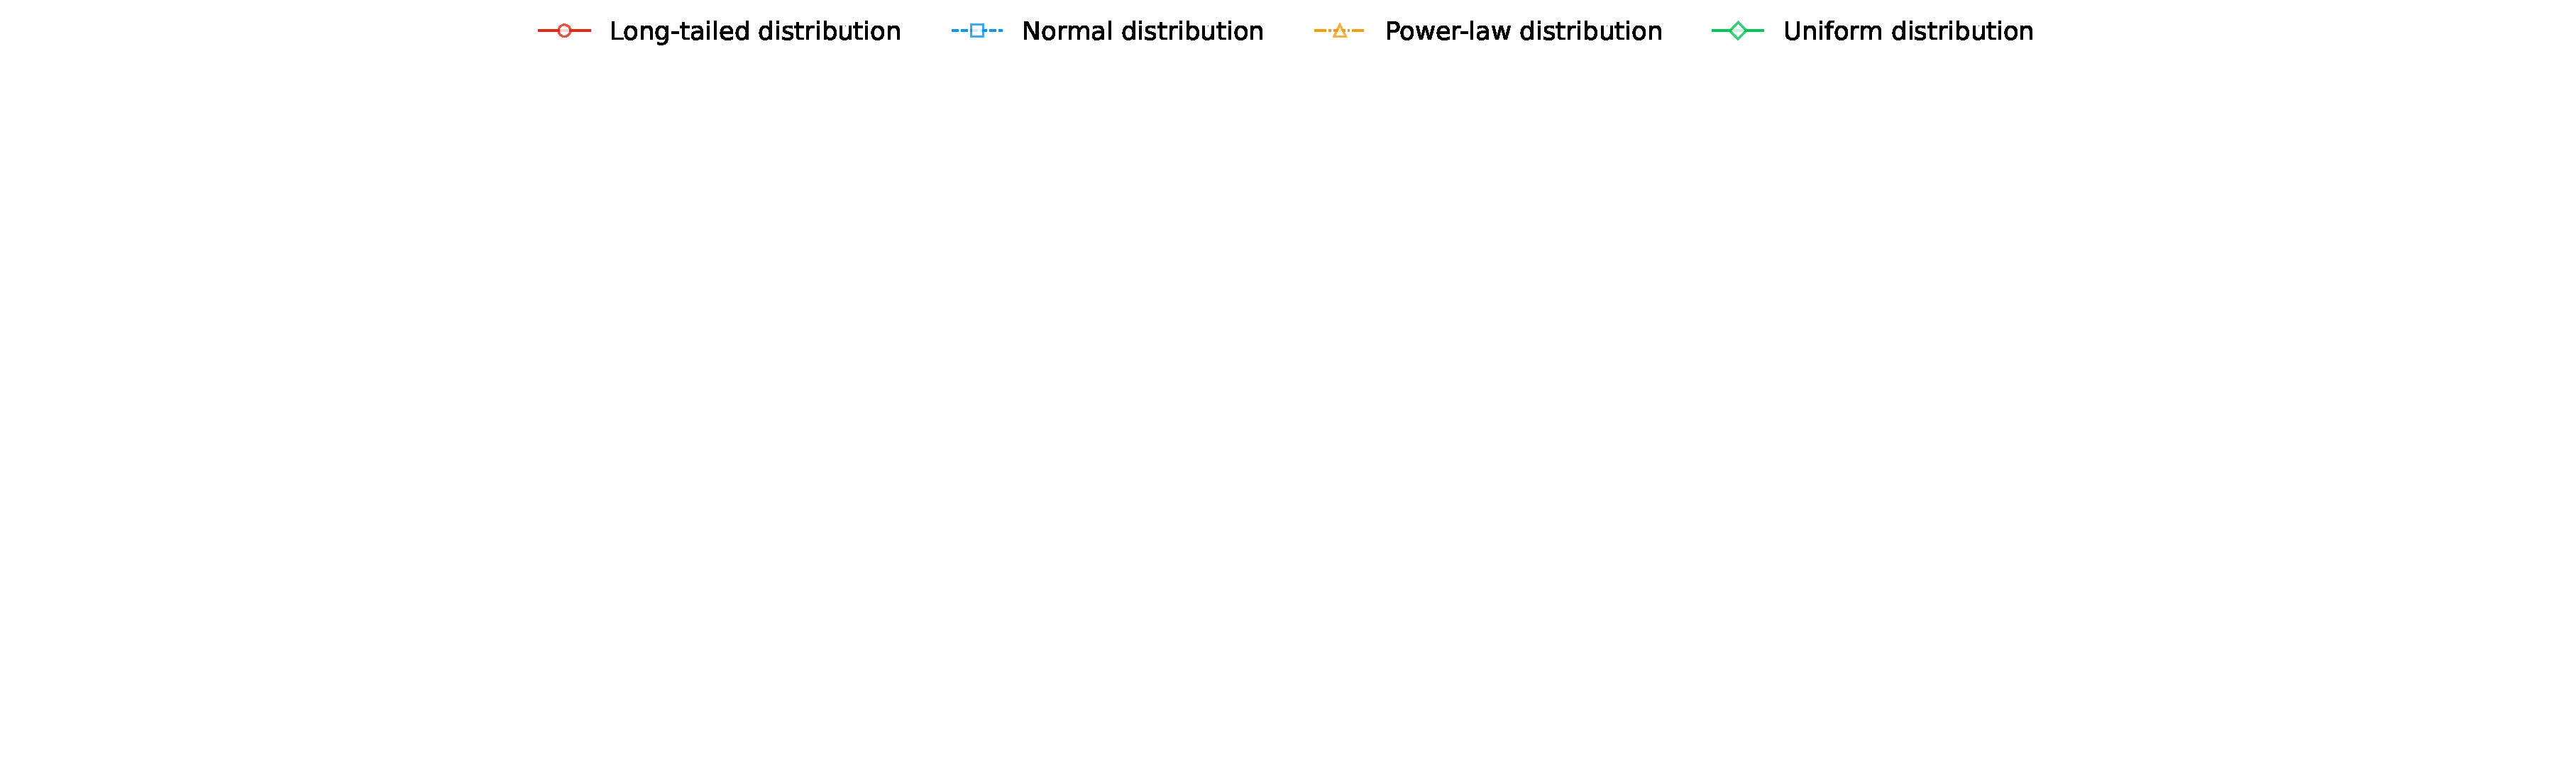
\includegraphics[width=\linewidth]{fig/exp_3_1_legend.pdf}
	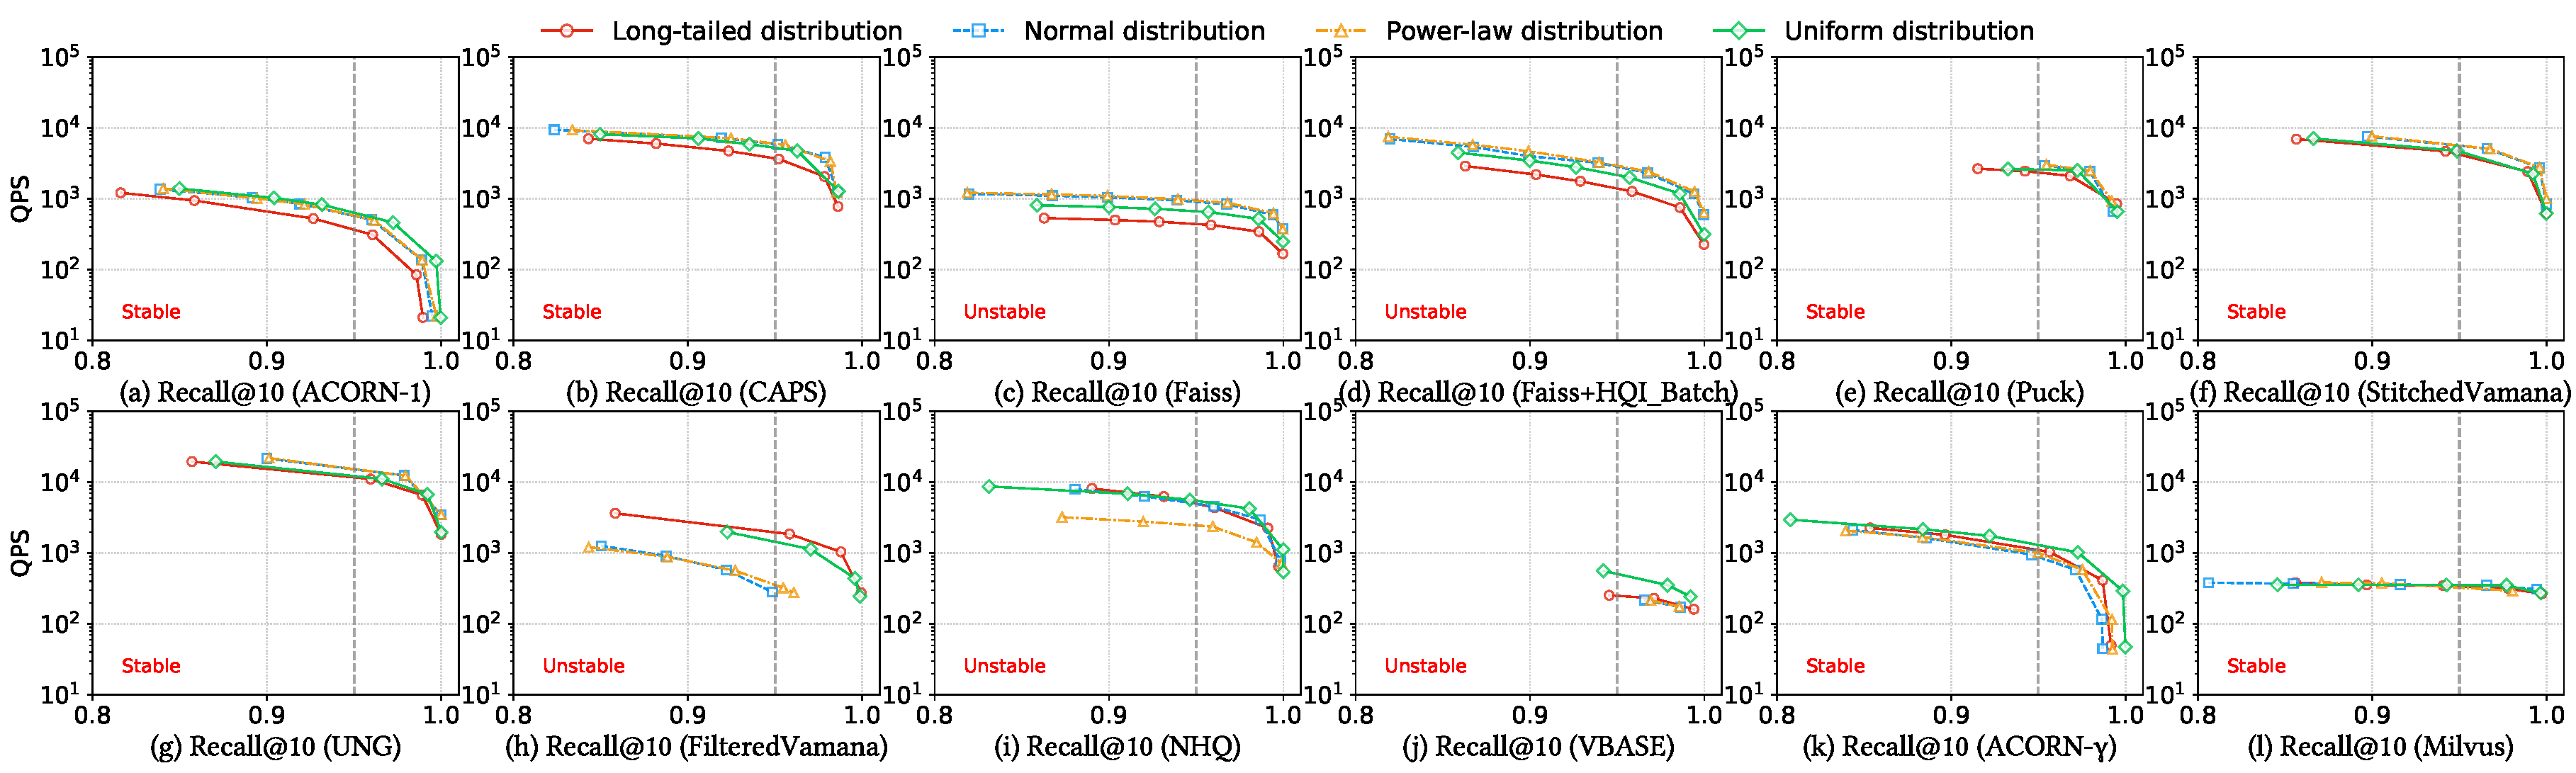
\includegraphics[width=\linewidth]{fig/exp_3_1.pdf}
	\caption{Effect of Attribute Distribution on Query Performance}
	\label{fig:attribute_distribution}
\end{figure*}

As shown in Figure~\ref{fig:attribute_selectivity} below, for performance under different attribute selectivity, to reflect the performance differences of each algorithm under different attribute selectivity, we added performance rankings for each algorithm across different selectivity levels in the figure. This provides a clearer illustration of how each algorithm is affected by different attribute selectivity.

%We also removed the  Figure~\ref{fig:attribute_selectivity_2}, which displayed too many algorithms in one plot and was difficult to interpret and somewhat redundant with Figure~\ref{fig:attribute_selectivity}. We believe these changes improve the clarity and readability of the paper, without reducing the completeness of the evaluation.




	\begin{figure*}
	\centering
	
	% 第一行:单独一张大图
	\begin{subfigure}{\textwidth}
		\centering
		
		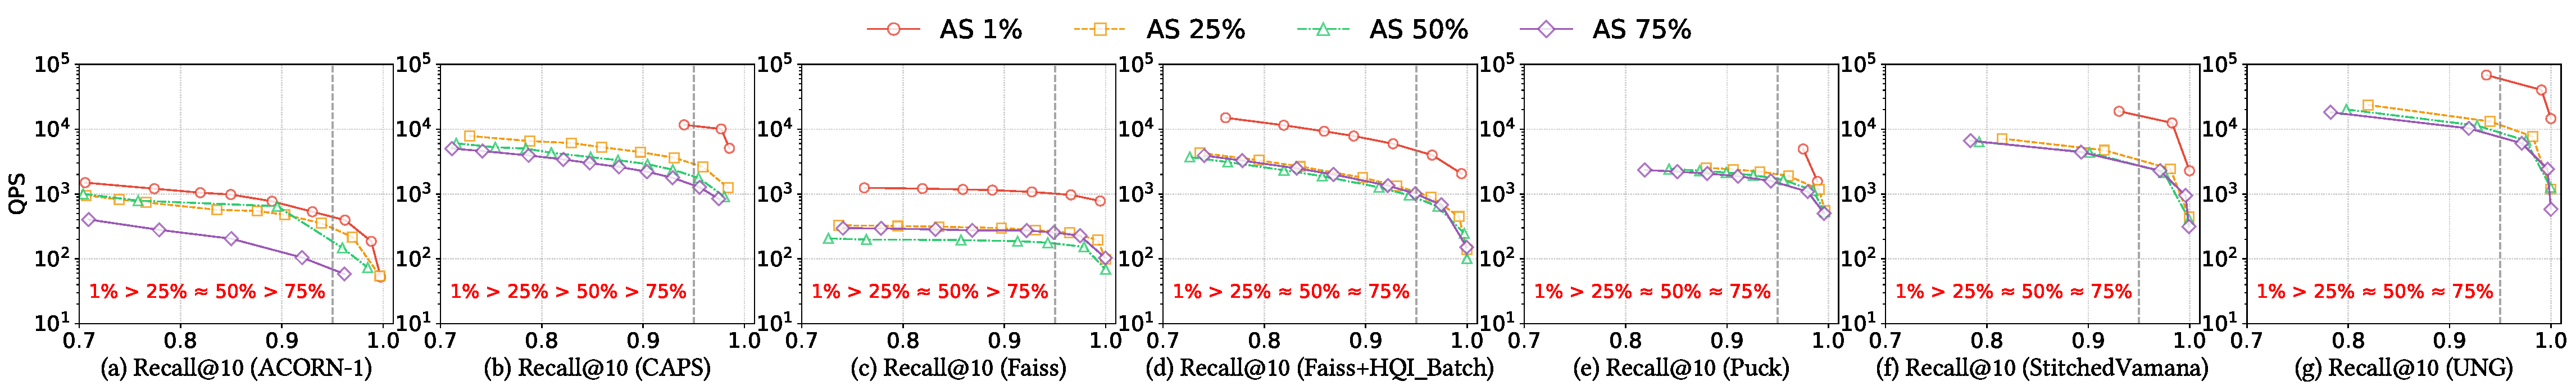
\includegraphics[width=0.95\textwidth]{fig/exp_5_2_1.pdf}
		\caption{Algorithms Optimized for Low AS}
		\label{fig:exp_5_2_1}
	\end{subfigure}
	
	\vfill % 增加垂直间距
	
	% 第二行:两张子图,左侧宽度是右侧的两倍
	\begin{subfigure}{0.627\textwidth} % 2/3 宽度
		\centering
		
		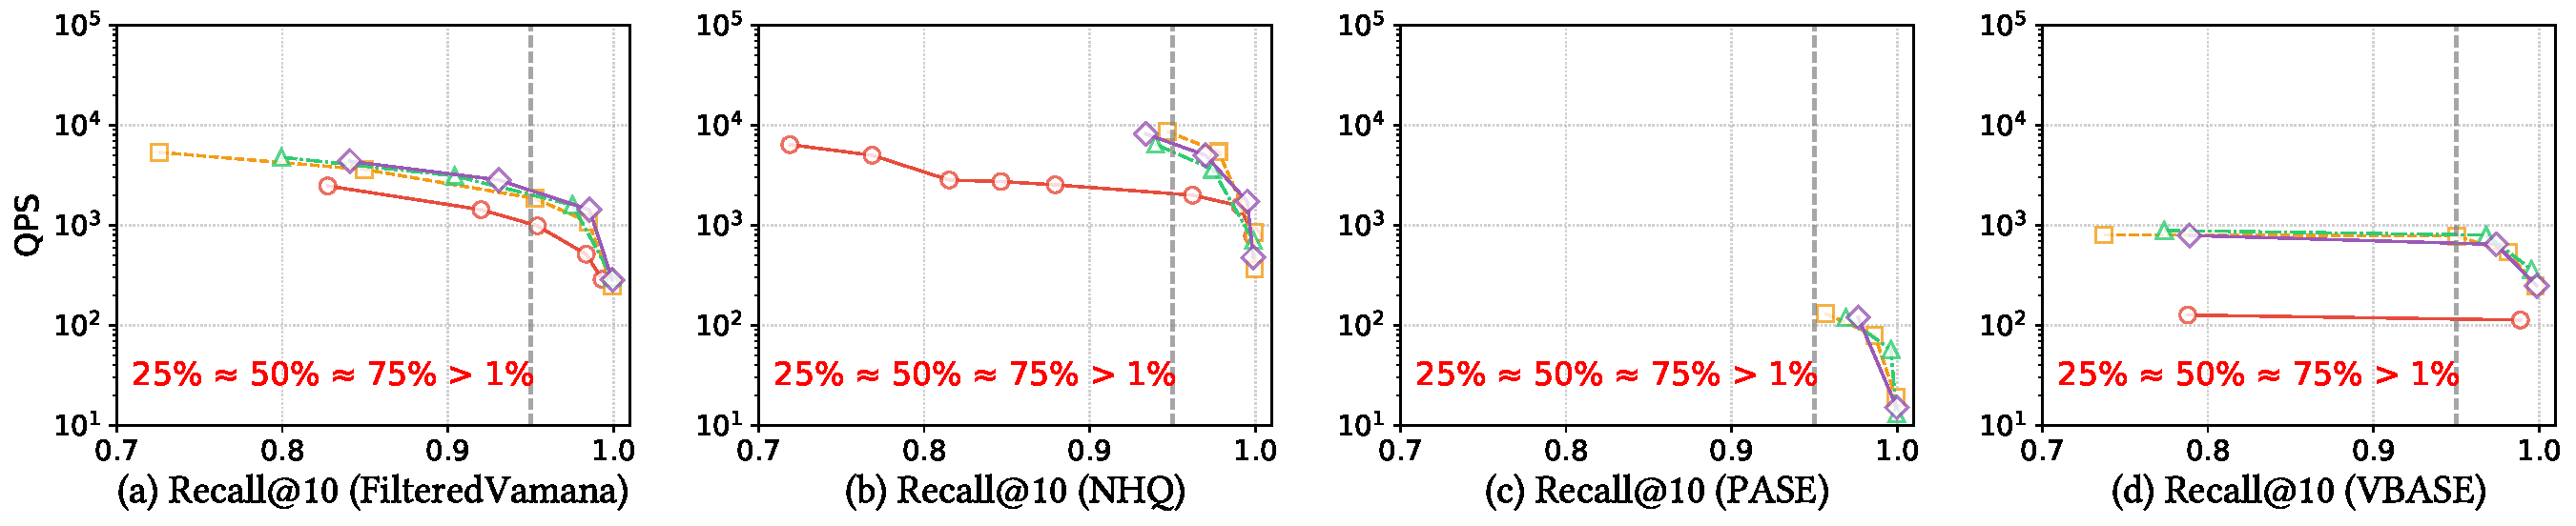
\includegraphics[width=0.96\textwidth]{fig/exp_5_2_2.pdf}
		\caption{Algorithms Optimized for High AS}
		\label{fig:exp_5_2_2}
	\end{subfigure}
	\hspace{1mm} % 增加水平间距
	\begin{subfigure}{0.33\textwidth} % 1/3 宽度
		\centering
		
		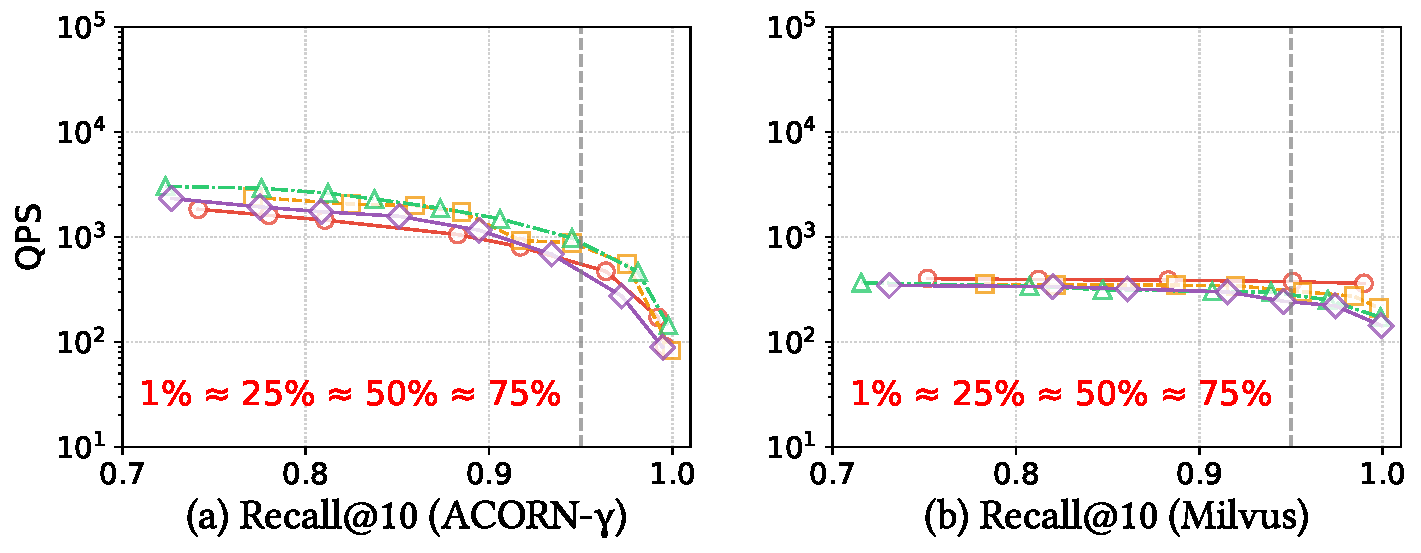
\includegraphics[width=0.96\textwidth]{fig/exp_5_2_3.pdf}
		\caption{Algorithms Insensitive to AS}
		\label{fig:exp_5_2_3}
	\end{subfigure}
	
	
	\caption{Performance of Different Attribute Selectivity (AS) under the Same Algorithm}
	\label{fig:attribute_selectivity}
\end{figure*}
%\begin{figure}[htbp]
%	\centering
%	%	
\includegraphics[width=0.8\linewidth]{fig/exp_5_2_1_legend.pdf}
%	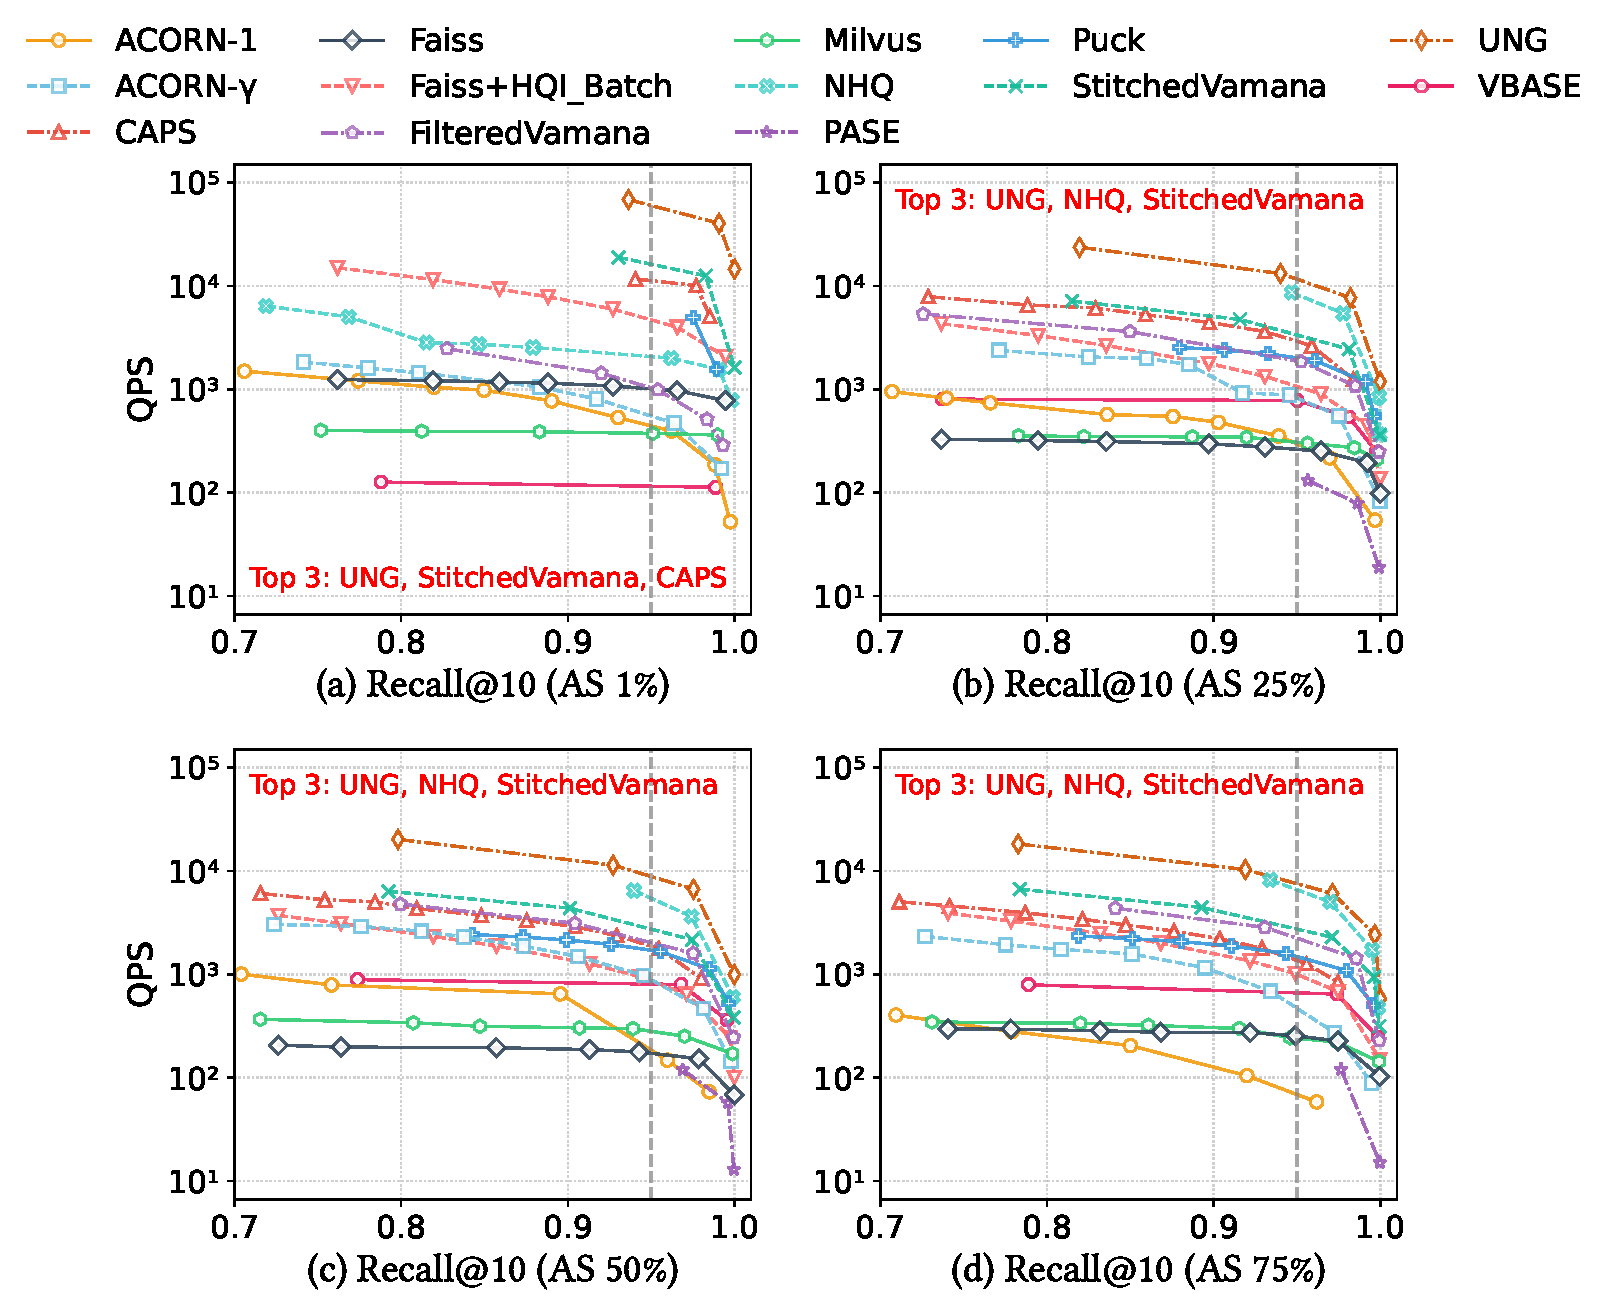
\includegraphics[width=\linewidth]{fig/exp_5_1_1_SingleLabel_1thread.pdf}
%	\caption{Different AS under the Same Algorithm}
%	\label{fig:attribute_selectivity_2}
%\end{figure}

%%%%%%%%%%%%%%%%%%%%%% R2 %%%%%%%%%%%%%%%%%%%%%%
\myfbox{
	\begin{metarevision}
		\textit{Run experiments with multi-modal queries (e.g., combining text and images) or more complex query types involving both attribute and range filters.}
	\end{metarevision}
}

\noindent
\textbf{Response:} We believe this is an excellent suggestion. To provide a more comprehensive evaluation of the robustness of each algorithm, we introduce new experiments on two challenging multi-modal datasets. 

First, we have incorporated a standard text-to-image dataset, which is widely adopted by existing multi-modal ANN algorithms. In this dataset, the base vectors are images while the query set consists of texts, creating a modality gap that demands stronger algorithm robustness to achieve good performance. Second, to further test performance on complex queries, we have constructed a more challenging dataset with a base set of 500,000 text vectors and 500,000 image vectors, and a query set containing 5,000 text and 5,000 image vectors. On this latter dataset, we perform both attribute filtering and range queries using combined text and image inputs to analyze the algorithm's robustness under more complex, mixed-modality conditions. The experimental results are shown in Figure~\ref{fig:attribute_multimodel} and Figure~\ref{fig:range_multimodel}.\textbf{ (Please see Section 4.1.1, Section 4.2.3 and Secntion 4.3.3, highlighted in blue in the revised manuscript.)  
	%Please refer to the blue highlighted parts in  Section 4.1.1 paragraph 4 and  Section 4.2.4 and Section 4.3.4 under Multi-modal Queries.)
}

As for complex query types that involve both attribute filtering and range queries simultaneously, to the best of our knowledge, existing algorithms—except for general-purpose systems such as Milvus and Faiss—do not support this functionality. For example, ACORN needs to build separate indexes for each scenario and cannot handle attribute filtering and range queries simultaneously. Therefore, we do not consider this type of complex query in our experiments but instead study the two query types separately. 

Section 4.1.1: \textcolor{blue}{
"Additionally, we use the Out-of-Distribution (OOD) dataset Text2Image and the large-scale dataset Deep100M to evaluate the generalization capability of the algorithms. The Text2Image dataset includes two versions. The original version contains 1 million image embeddings as the base dataset and uses 10 thousand text embeddings as the query set. The Text2Image-Mix version is composed of 0.5 million image embeddings and 0.5 million text embeddings as the base dataset, with a query set of 5 thousand image embeddings and 5 thousand text embeddings."
}

Section 4.2.3: \textcolor{blue}{
	"We conduct experiments on two multimodal datasets Text2image-Mix and Text2image. On Text2imageMix dataset, as shown in Figure 9, UNG and NHQ consistently perform best, followed by CAPS. Although the dataset contains two modalities, due to the significant differences between the modalities, they are actually two separate regions in the vector space. The performance is similar to that of the single-modal dataset in Figure 4. This is because mixed multi-modal queries are actually the same as conducting experiments on two datasets of the same modality. This is not actually a difficult query. In contrast, the Text2image dataset shown in Figure 9 is different. The query set and the base dataset belong to two completely different modalities. Queries are far from the dataset points, and the ground truths are more dispersed. To find the ground truths, algorithms typically need to examine more points, which leads to degraded performance." 
}

Section 4.3.3: \textcolor{blue}{
		"Similar to attribute filtering, the performance of range filtering queries on the Text2image-Mix dataset (Figure 14) is similar to the single-modality query performance (Figure 13). However, on the Text2Image dataset, these algorithms exhibit a significant performance degradation (Figure 14). This is because most of these range query algorithms are graph-based, and such algorithms require more iterations to find true neighbors in OOD datasets."
}

\begin{figure}[htbp]
	\centering
	
\includegraphics[width=0.95\linewidth]{fig/attribute_legend.pdf}
	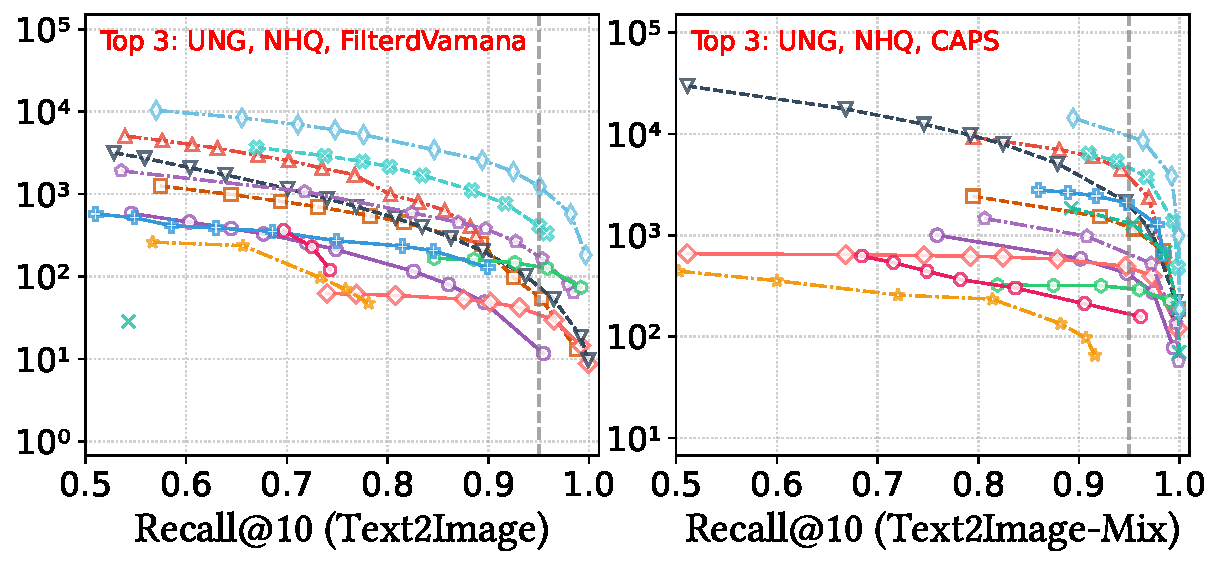
\includegraphics[width=\linewidth]{fig/attribute_multimodel_2.pdf}
	\caption{Multi-modal Datasets (AF)}
	\label{fig:attribute_multimodel}
\end{figure}

\begin{figure}[htbp]
	\centering
	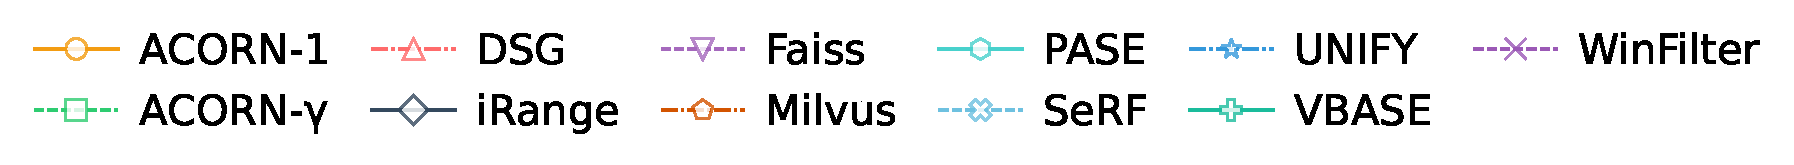
\includegraphics[width=0.95\linewidth]{fig/range_legend.pdf}
	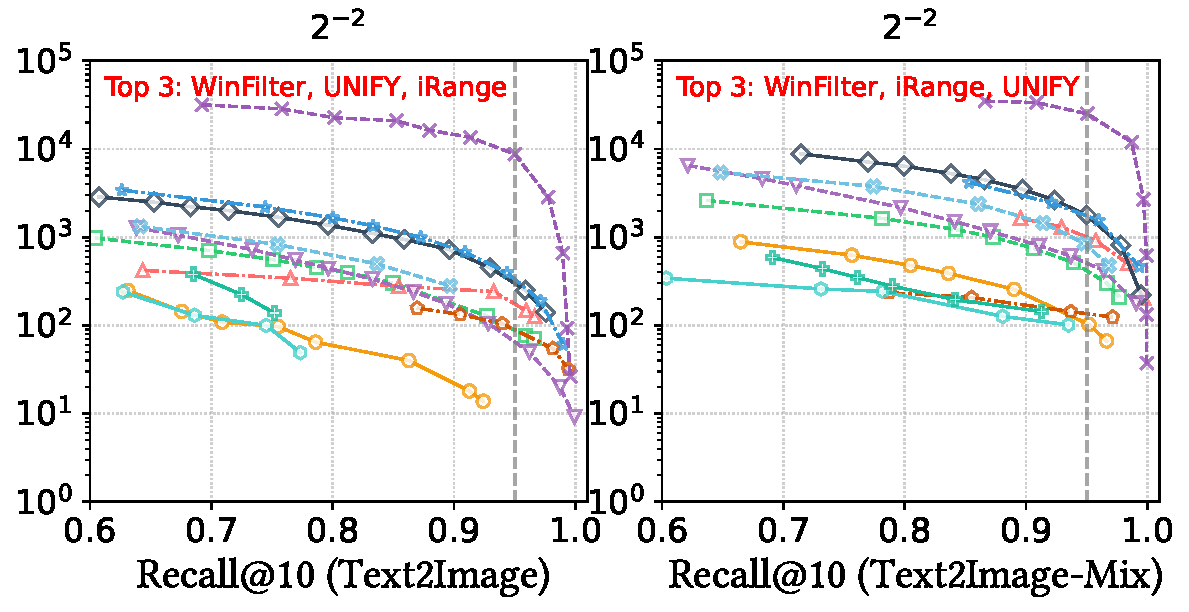
\includegraphics[width=\linewidth]{fig/range_multimodel_2.pdf}
	\caption{Multi-modal Datasets (RF)}
	\label{fig:range_multimodel}
\end{figure}

%\begin{figure}[t]
%	\centering
%	
%	% 上面的图例,居中并可通过 hspace 调整左右位置
%	\hspace*{8pt} % 可调整的参数,负值左移,正值右移,例如 -20pt 或 20pt
%	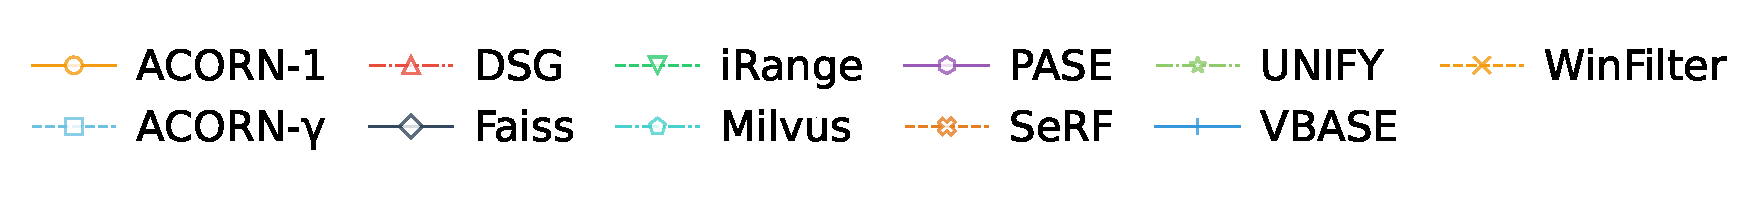
\includegraphics[width=0.9\columnwidth]{fig/range_2_2_legend.pdf} % 图例图片路径
%	
%	% --- 不再使用 subfigure ---
%	% 直接放置第二张图片,可以加一点垂直间距
%	\vspace{5pt} 
%	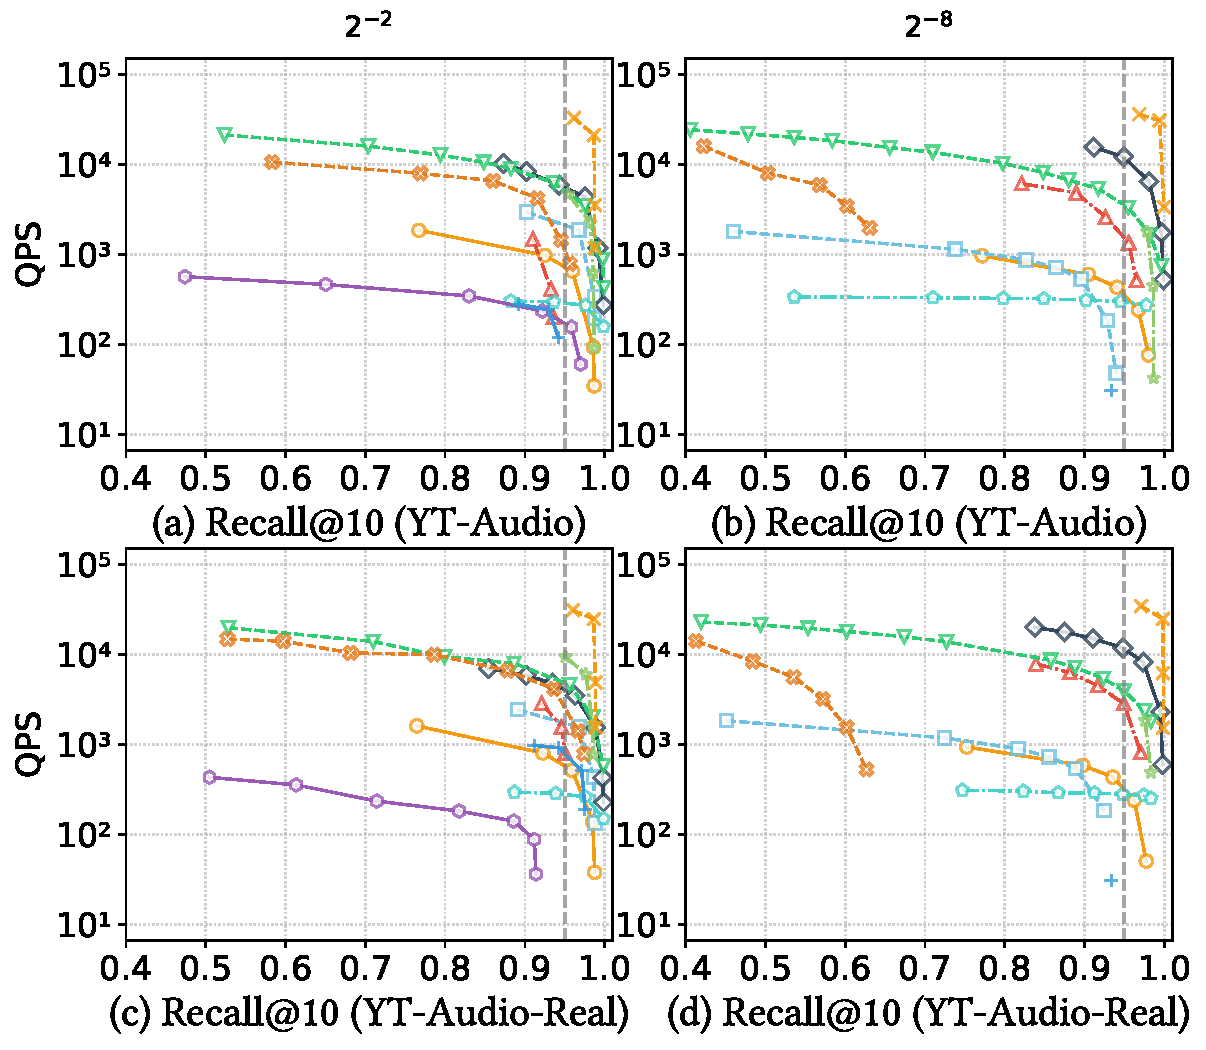
\includegraphics[width=0.95\columnwidth]{fig/range_2_2.pdf}
%	
%	\caption{Comparison of Real and Synthetic Attributes}
%	\label{fig:range_2_2}
%	
%\end{figure}


%%%%%%%%%%%%%%%%%%%%%% R4 %%%%%%%%%%%%%%%%%%%%%%
\myfbox{
	\begin{metarevision}
		\textit{Instead of using the point ID, run experiments with meaningful attributes for RF-NN search on datasets (Deep, YT-Audio, WIT).}
	\end{metarevision}
}

\noindent
\textbf{Response:} 
Thank you for your suggestion. Using ID as an attribute is a prevalent method in current range filtering algorithm evaluations, so we also use ID as attributes in our experiments. To conduct a meaningful evaluation, we have updated two of our datasets (YT-Audio-Real, WIT-Real) to include real attributes.  \textbf{(Please see Section 4.1.1, highlighted in blue in the revised manuscript.)}



\textcolor{blue}{
	"WIT-Real and YT-Audio-Real datasets use real attributes. For the WIT-Real dataset, we use the CLIP model to encode the page title into vectors, and extract the language type and the length of the context page description as real attributes. The YT-Audio-Real dataset uses YouTube8M data, employing the video category ID and view counts as real attributes for this dataset."
}
%%%%%%%%%%%%%%%%%%%%%% R5 %%%%%%%%%%%%%%%%%%%%%%


\myfbox{
	\begin{metarevision}
		\textit{Evaluate if the server setting affects the relative ordering of methods in experiments}
	\end{metarevision}
}

\noindent
\textbf{Response:} 
That is a great suggestion. In order to figure out if the server setting affects the relative ordering of methods, we conducted additional experiments on an Ubuntu 20.04 server equipped with dual Intel(R) Xeon(R) Gold 6330 CPUs @ 2.00GHz featuring 128GB of RAM and 84 MiB of L3 cache using the YT-Audio-Real dataset. The experimental results of attribute filtering and range filtering are shown in Figure~\ref{fig:attribute-cross-platform} and Figure~\ref{fig:range-cross-platform}, respectively.
The results show that the performance differences across algorithms remain small, and their relative rankings do not change significantly across servers.
We did observe slightly lower QPS on this server compared to our original one, which is mainly due to the the lower CPU frequency, reduced RAM capacity, and smaller L3 cache of the Xeon 6330 processors. \textbf{(Please see Section 4.2.3 and Section 4.3.3, highlighted in blue in the revised manuscript.)} 

Section 4.2.3:
%\textcolor{blue}{"To investigate the impact of different server configurations on the performance of the algorithms, we conduct additional experiments on a server equipped with dual Intel(R) Xeon(R) Gold 6330 CPUs @ 2.00GHz using the YT-Audio-Real dataset, and the results are shown in Figure 12b. Compared with the experimental results on the original server, the relative ranking of the algorithms remains largely unchanged, indicating that the performance of these methods is not significantly affected by differences in CPU configurations. Due to the lower CPU frequency and smaller RAM capacity, the QPS values are slightly lower across all methods."}
\textcolor{blue}{"To investigate the impact of different server configurations on the performance of the algorithms, we conduct additional experiments on an Ubuntu 20.04 server equipped with dual Intel(R) Xeon(R) Gold 6330 CPUs @ 2.00GHz featuring 128GB of RAM and 84 MiB of L3 cache using the YT-Audio-Real dataset, and the results are shown in Figure 10. It is not difficult to see that the relative ranking of the algorithms under the two servers essentially remains unchanged, indicating that the performance of these methods is not significantly affected by differences in CPU configurations. Due to the lower CPU frequency, reduced RAM capacity, and smaller L3 cache, all methods demonstrate slightly lower QPS values."}

Section 4.3.3:
\textcolor{blue}{"Consistent with Section 4.2.3, we conduct range filtering experiments on the YT-Audio-Real dataset using two server configurations, with results presented in Figure 15. Although the third-ranked algorithm differs, we consider the ranking order remains stable since the performance of the third and fourth algorithms is comparable. Therefore, different server configurations only affect the performance of individual algorithms, with minimal impact on their relative performance ranking."}

\begin{figure}[htbp]
	\centering
	
\includegraphics[width=0.48\textwidth]{fig/attribute_legend.pdf}
	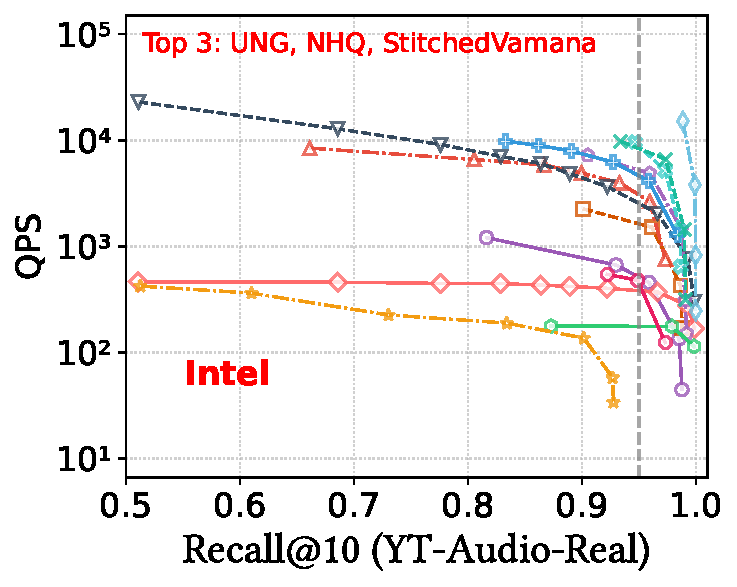
\includegraphics[width=0.495\linewidth]{fig/attribute_85.pdf}
	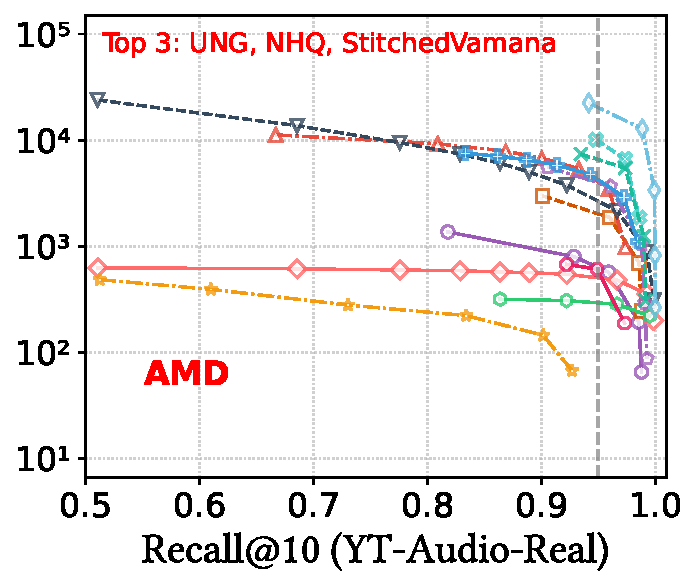
\includegraphics[width=0.47\linewidth]{fig/attribute_71.pdf}
	\caption{Different Platforms (AF)}
	\label{fig:attribute-cross-platform}
\end{figure}

\begin{figure}[htbp]
	\centering
	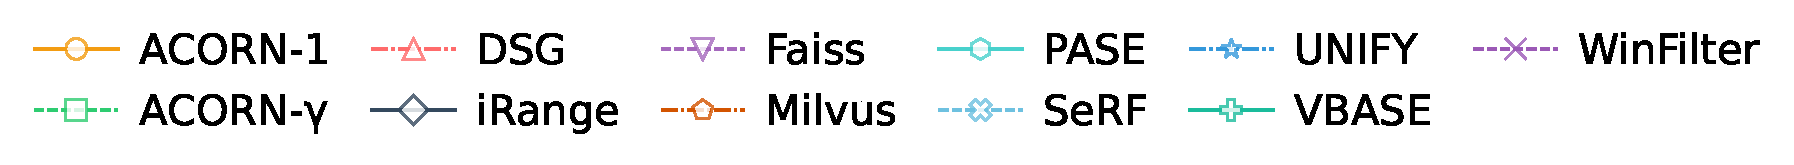
\includegraphics[width=0.48\textwidth]{fig/range_legend.pdf}
	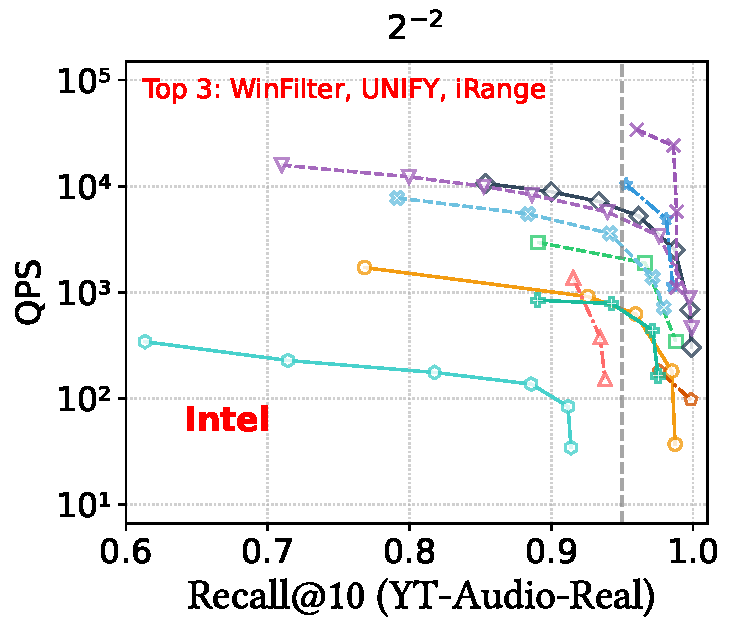
\includegraphics[width=0.495\linewidth]{fig/range_85.pdf}
	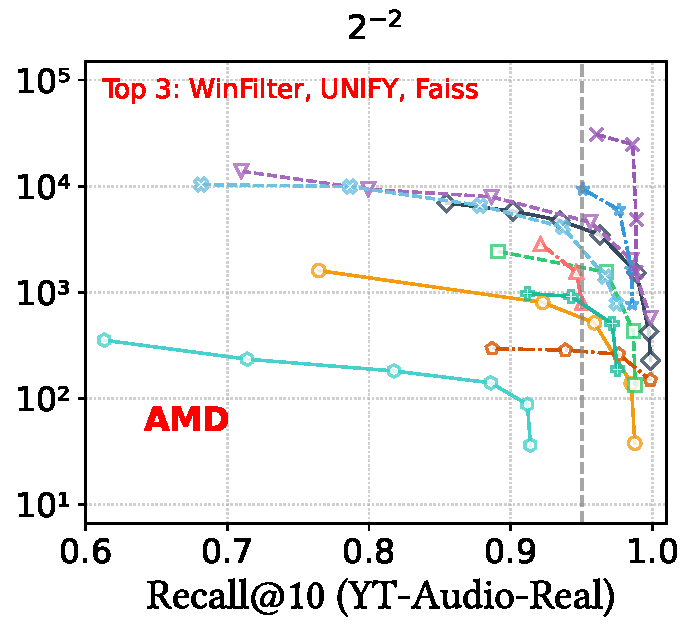
\includegraphics[width=0.47\linewidth]{fig/range_71.pdf}
	\caption{Different Platforms (RF)}
	\label{fig:range-cross-platform}
\end{figure}

%%%%%%%%%%%%%%%%%%%%%% R6 %%%%%%%%%%%%%%%%%%%%%%
\myfbox{
	\begin{metarevision}
		\textit{In Table 1, please clarify which methods are disk-based, and which methods are memory-based.
			For disk-based methods, it is also meaningful to report the cost breakdown (e.g., in terms of I/O time and CPU time).}
	\end{metarevision}
}

\noindent
\textbf{Response:} 
Thank you for your suggestion. Currently, except for Filtered-DiskANN, other hybrid query methods are memory-based, so we added the characteristic of whether to support disk for each algorithm in Table \ref{tab:compair_1}, which corresponds to Table 1 in the original paper.
\begin{figure}[htbp]
	\centering
	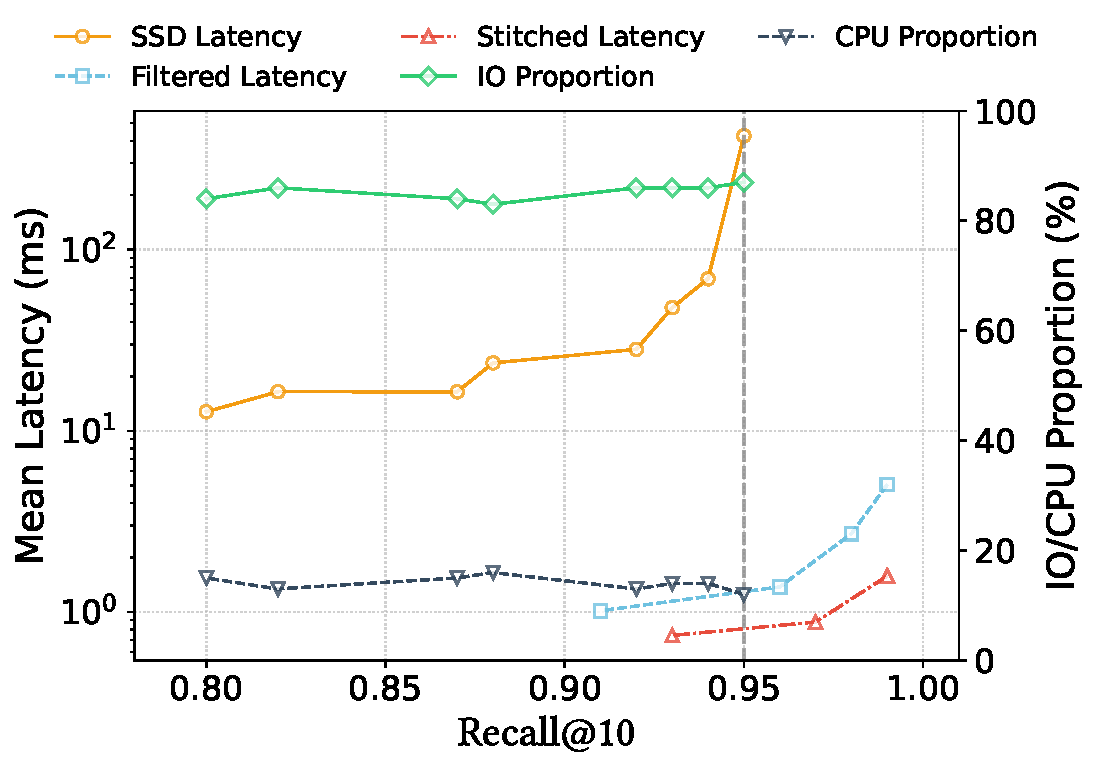
\includegraphics[width=\linewidth]{fig/recall_latency_all.pdf}
	\caption{Performance Comparison of SSD-Based and In-Memory Execution of FilteredDiskANN}
	\label{fig:recall-latency}
\end{figure}

 To analyze the cost breakdown of disk-based methods in greater detail, we also compared the search performance difference of Filtered-DiskANN on memory and SSD using real data sets. 
We conducted additional experiments on the YT-Audio-Real dataset, comparing three variants of DiskANN.
(1) SSD-based Filtered-DiskANN (original disk-based method);
(2) FilteredVamana (memory-based method);
(3) StitchedVamana (memory-based method).
We have run all experiments with 32 search threads for fair comparison. Figure~\ref{fig:recall-latency} shows the mean latency (log-scale, left y-axis) and I/O vs CPU proportion (right y-axis) across different Recall\@10 levels:

%\begin{itemize}
%	\item SSD-based FilteredDiskANN (original disk-based method)
%	\item FilteredVamana (memory-based method)
%	\item StitchedVamana (memory-based method)
%\end{itemize}

Latency-Recall Tradeoff:
As expected, SSD-based Filtered-DiskANN exhibits significantly higher latency than in-memory methods, especially at higher recall levels. When Recall@10 reaches 0.96, its latency increases super-linearly to over 100 ms.

Cost Breakdown of Filtered-DiskANN:The I/O proportion consistently dominates, maintaining 80\%–85\% of the total latency even at different recall levels.
The CPU proportion remains low (10–15\%), indicating that I/O is the major bottleneck in disk-based search pipelines.
This clearly shows that improving disk read efficiency or reducing I/O volume is critical for performance optimization.

In-memory Methods:
FilteredVamana achieves a good balance, staying under 30 ms while achieving Recall@10 > 0.97.
While StitchedVamana achieves extremely low latency (sub-5 ms) due to its stitched multi-label index structure, its fixed edge connectivity may limit effectiveness under highly uncorrelated label distributions. Nevertheless, it consistently supports 90\%+ Recall@10 across diverse datasets, as shown in our evaluations.

\textbf{Note: }Due to space limitations and the fact that only one method supports disk-based execution, we did not include the above experiments and analysis in the revised paper.

%%%%%%%%%%%%%%%%%%%%%% R7 %%%%%%%%%%%%%%%%%%%%%%
\myfbox{
	\begin{metarevision}
		\textit{Report the peak memory usage of query processing.}
	\end{metarevision}
}

\noindent
\textbf{Response:} 
We believe your suggestion is very reasonable, and the experiment on search peak memory is indeed an important component. We are deeply aware of this shortcoming, so we provide the search peak memory usage of each algorithm in the time and space overhead section and carefully analyze the reasons. We present the search peak memory usage for the newly added attribute filtering and range filtering in Figure \ref{fig:search_memory_mb_comparison} and Figure \ref{fig:rangeFilter_search_memory_mb}, respectively.
\textbf{(Please see Section 4.2.1 and Section 4.3.1, highlighted in blue in the revised manuscript.)}
\begin{figure}[htbp]
	\centering
	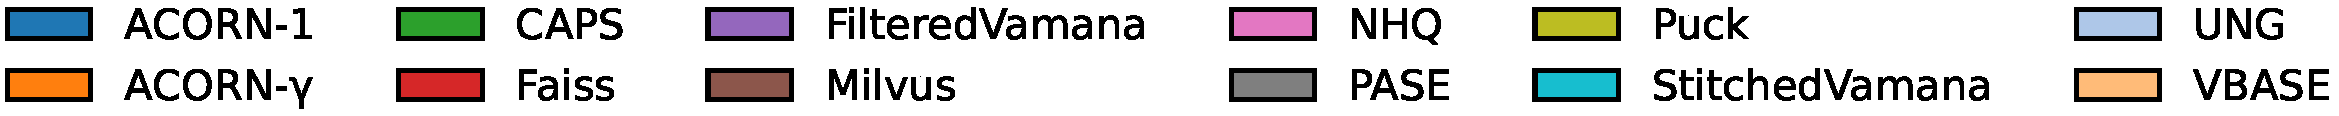
\includegraphics[width=\linewidth]{fig/legend_only.pdf}
	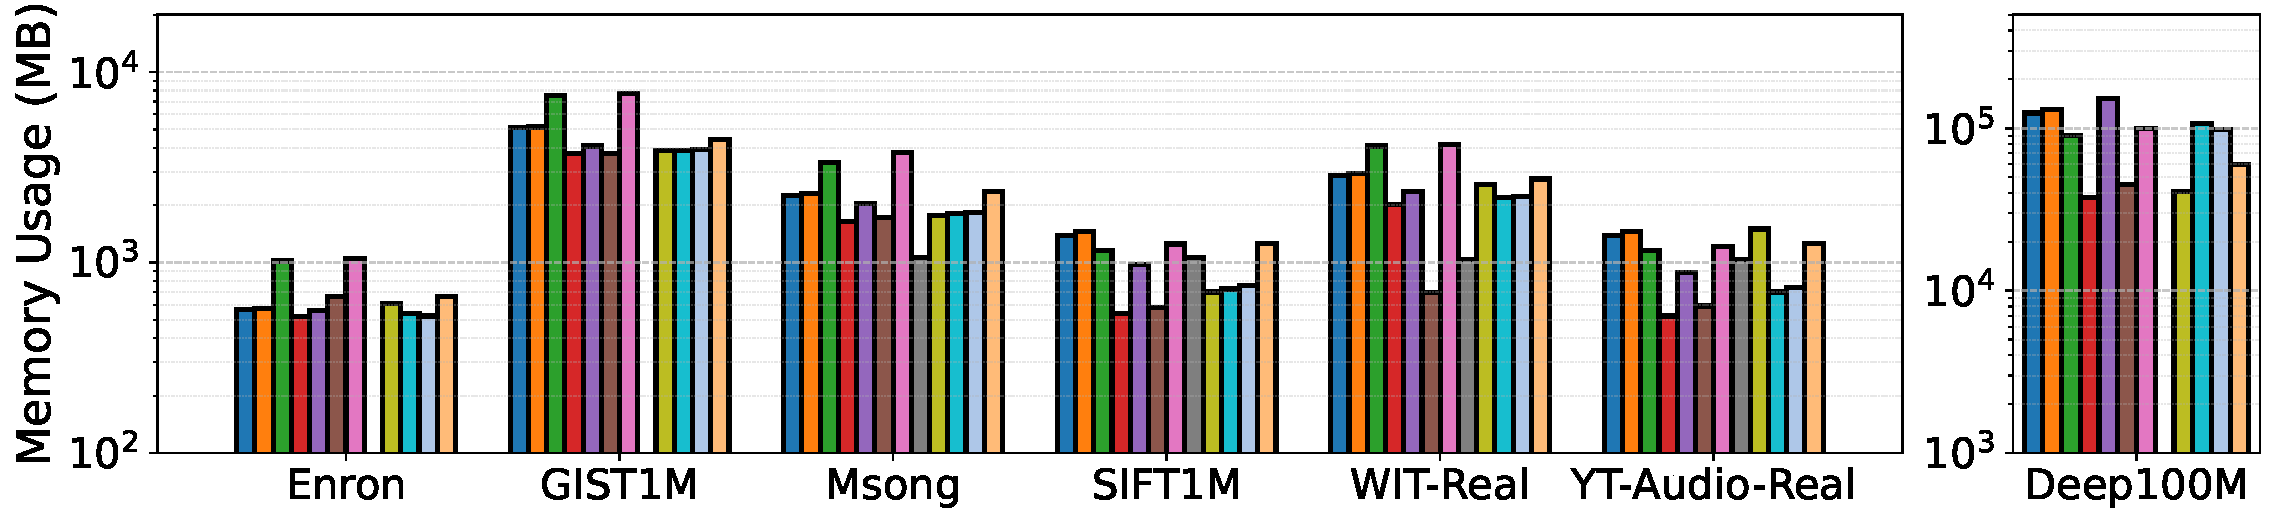
\includegraphics[width=\linewidth]{fig/searchMem/label_memory_comparison.pdf}
	\caption{Attribute Filtering Search Peak Memory}
	\label{fig:search_memory_mb_comparison}
\end{figure}

\begin{figure}[htbp]
	\centering
	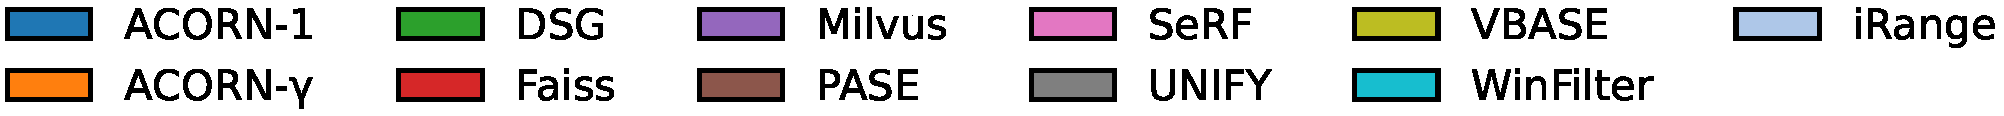
\includegraphics[width=\linewidth]{fig/rangeFilter_legend_only.pdf}
	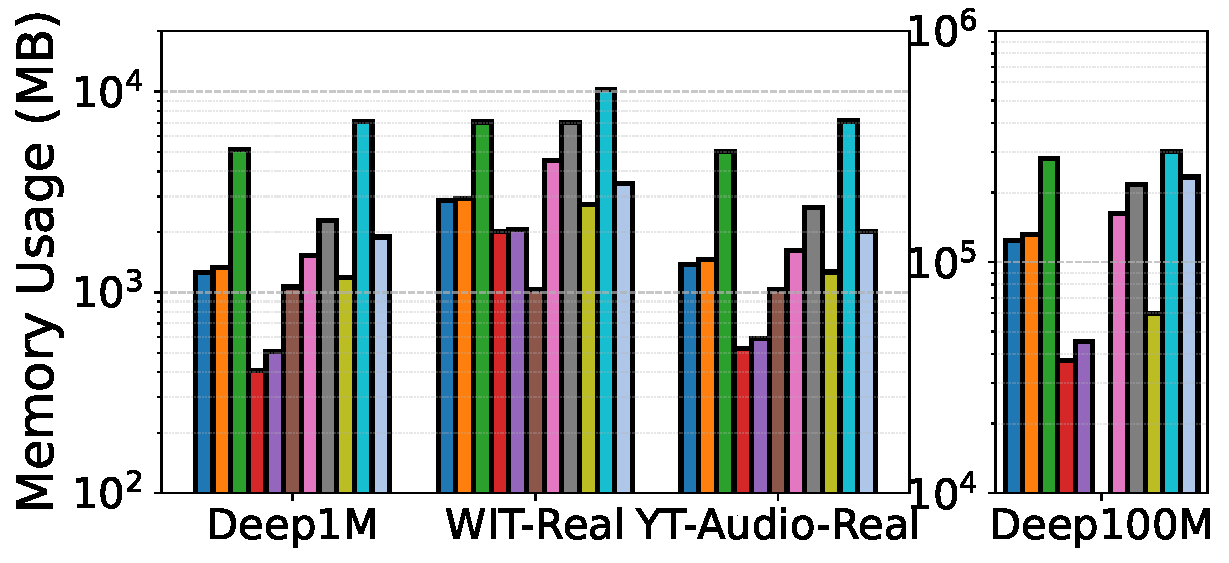
\includegraphics[height=2.5cm]{fig/searchMem/range_memory_comparison.pdf}
	\caption{Range Filtering Search Peak Memory}
	\label{fig:rangeFilter_search_memory_mb}
\end{figure}



%For attribute filtering, please see section 4.2.1.
% \textbf{(Please refer to the blue highlighted parts in Section 4.2.1 for attribute filtering.)}
Section 4.2.1:
\textcolor{blue}{\textit{\textbf{"Peak memory.}}	
	We present the peak memory usage during index construction and query processing in Figure 3c and Figure 3d, respectively. We observe that peak memory usage is generally correlated with the combined size of the index and the dataset. Methods that produce larger indexes tend to consume more memory during both construction and querying, and this trend holds consistently across different datasets.}

\textcolor{blue}{However, there are notable exceptions. During index construction, PASE adopts an on-demand loading strategy, resulting in build peak memory usage even lower than the final index size. NHQ generates a large number of candidate neighbors during construction but retains only a small subset per node in the final index, leading to high peak memory usage despite a relatively compact index.
During querying, CAPS maintains a large candidate set dynamically, which significantly increases its search peak memory consumption."}

%For range filtering, please see section 4.3.1.
 %\textbf{(Please refer to the blue highlighted parts in Section 4.3.1 for range filtering.)}
 Section 4.3.1:
\textcolor{blue}{\textit{\textbf{"Peak memory.}}  
	As explained in the attribute filtering analysis, methods with larger index sizes (including the dataset) tend to exhibit higher peak memory consumption. As shown in Figure12c and Figure12d, range filtering also adheres to this pattern.}  

	
	\textcolor{blue}{WinFilter also presents an exception:  its peak memory usage is also affected by the level of parallelism. Although the final index size remains relatively small, the peak memory usage increases significantly during both construction and search. During construction, this is caused by the parallel building of local indices for each tree node, which results in substantial temporary memory usage. Similarly, during search, WinFilter needs to load multiple local indices in parallel for different tree nodes, further contributing to high peak memory consumption."}


%%%%%%%%%%%%%%%%%%%%%% R8 %%%%%%%%%%%%%%%%%%%%%%
\myfbox{
	\begin{metarevision}
		\textit{Run Scalability experiments with larger datasets.}
	\end{metarevision}
}

\noindent
\textbf{Response:} 
Thank you for your valuable suggestion regarding our experiments. In Section 4.2.3 and Section 4.3.3, we have added experiments on the Deep100M dataset. The results show that most algorithms struggle to balance performance with time and space costs on this large-scale dataset. In particular, StitchedVamana performs poorly on Deep100M. The experimental results are shown in Figure~\ref{fig:attribute big dataset} and Figure~\ref{fig:range big dataset}. \textbf{(Please see the "Large-scale Datasets" part of Section 4.2.3 and Section 4.3.3, highlighted in blue in the revised manuscript.)}
%\textbf{(Please refer to the blue highlighted parts in Section 4.2.4 and Section 4.3.4 under Large-scale Datasets.)}


Section 4.2.3:\textcolor{blue}{"As shown in the Figure 11, on the 100M dataset, UNG and NHQ still exhibit excellent performance, demonstrating good adaptability to large-scale datasets. However, this also comes with significant memory overhead. The clustering-based algorithm Faiss+HQI\_Batch shows moderate performance but has very low memory overhead, which also has certain practical significance. Furthermore, we do not present the results of StitchedVamana and CAPS, as their recall remained consistently low. StitchedVamana sets the search entry point to 0 by default, which makes it prone to getting stuck in local optima when the entry is far from the target region, hindering effective navigation. CAPS, on the other hand, cannot properly run large-scale dataset experiments because its code implementation does not account for such scenarios."}

Section 4.3.3:
\textcolor{blue}{"As shown in the Figure 16, On the deep100M dataset, the top 3 ranked algorithms (WinFilter, UNIFY, and iRange) remain unchanged. However, their high performance is achieved at the cost of extremely high memory consumption (Figure 12d). In contrast, VBASE and Faiss demonstrate moderate performance while consuming significantly less memory."}


\begin{figure}[htbp]
	\centering
	
\includegraphics[width=0.95\linewidth]{fig/attribute_legend.pdf}
	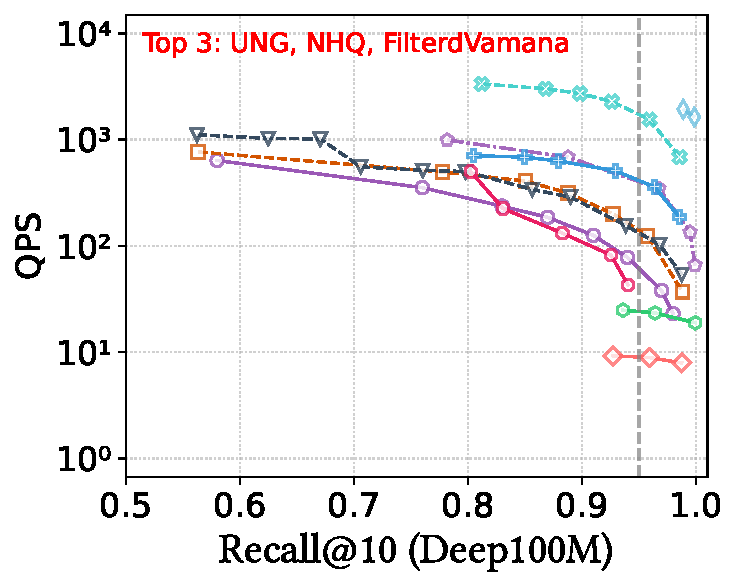
\includegraphics[width=0.7\linewidth]{fig/attribute_100M.pdf}
	\caption{Large-Scale Dataset (AF)}
	\label{fig:attribute big dataset}
\end{figure}

\begin{figure}[htbp]
	\centering
	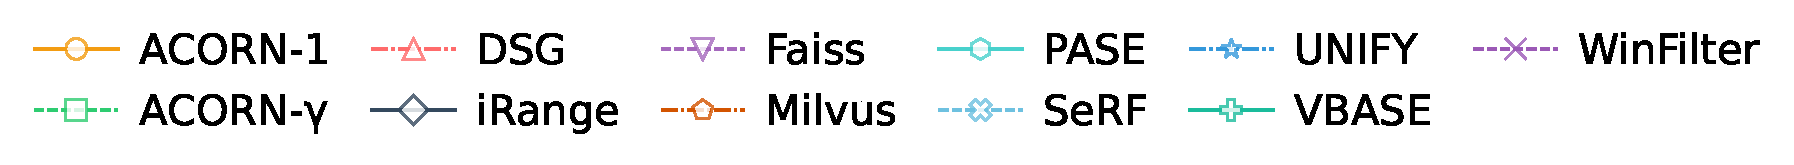
\includegraphics[width=0.95\linewidth]{fig/range_legend.pdf}
	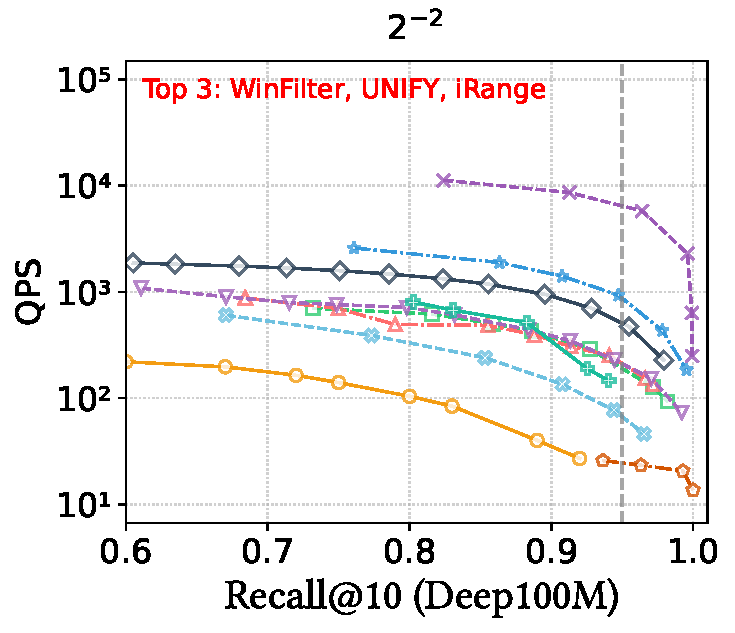
\includegraphics[width=0.7\linewidth]{fig/range_deep100M.pdf}
	\caption{Large-Scale Dataset (RF)}
	\label{fig:range big dataset}
\end{figure}


%%%%%%%%%%%%%%%%%%%%%% R9 %%%%%%%%%%%%%%%%%%%%%%
\myfbox{
	\begin{metarevision}
		\textit{Clearer insights and guidelines wrt the strength and weaknesses of the compared system.}
	\end{metarevision}
}

\noindent
\textbf{Response:} 
%Thank you for your valuable suggestion. We agree that our previous analysis of the strengths and weaknesses of the algorithms was not sufficiently clear.
%
%To address this, we add a summary table that provides a clearer and more structured comparison of the strengths and weaknesses of each algorithm, offering deeper insights and more concrete guidelines for understanding their trade-offs.
Thank you very much for your insightful comments.  We have revised the discussion section to provide a detailed analysis of the pros and cons of each algorithm, along with an in-depth examination of their internal mechanisms to uncover the fundamental reasons behind their performance.
\textbf{(Please see Section 5.1.1, Section 5.1.2 and Section 5.1.3, highlighted in blue in the revised manuscript.)}

Section 5.1.1:\textcolor{blue}{
	"Overall, UNG, NHQ and FilteredDisk-ANN demonstrate strong performance. However, UNG suffers from performance degradation when the attribute count differs between indexing and querying. NHQ, due to its distance fusion design, also experiences performance drops when there is a significant mismatch in attribute numbers between indexing and querying, and its performance is sensitive to attribute distribution. }

\textcolor{blue}{The two variants of Filtered-DiskANN (FilteredVamana and StitchedVamana) support only single-attribute queries and multi-attribute OR queries. FilteredVamana supports dynamic insertion and disk-based indexing, making it suitable for memory-constrained scenarios. However, its disk-based construction significantly increases indexing time, and its performance is highly sensitive to attribute distribution. In contrast, StitchedVamana offers better search performance but performs poorly on 100M-scale datasets and OOD datasets.}

\textcolor{blue}{
	CAPS, based on clustering, features low index space overhead. It offers flexible support for varying numbers of attributes and is optimized for low-selectivity attribute scenarios, but its overall performance is relatively moderate.
	Puck is well-suited for large-scale datasets such as those with 100 million points. It offers fast index construction and low memory consumption in such scenarios. "}


Section 5.1.2: \textcolor{blue}{
	"WinFilter achieves the best search performance but requires high time and memory resources during index construction. For large-scale datasets (e.g., with 100 million points), parameter tuning—particularly of tree height—is needed to prevent excessive index growth. When QPS and recall are not strict requirements, its basic variant, Vamana-WST, offers a more efficient alternative with significantly lower indexing overhead.
}

\textcolor{blue}{
	iRange has relatively low time and space costs for index construction. However, its search performance declines significantly with increasing query range. Despite offering threading parameters for indexing, it does not effectively utilize multi-core parallelism in practical scenarios.
	SeRF incurs low time and space overhead but achieves only moderate overall query performance, with notably weaker results in small-range query scenarios.
	DSG supports unordered dynamic insertions and range queries, but its index construction is limited to single-threaded execution, resulting in long build times and poor practical applicability.}

\textcolor{blue}{
	UNIFY adopts multiple filtering strategies tailored to different query range sizes, avoiding the limitations of a single strategy in specific scenarios. It requires only one index to support all queries, allows dynamic insertions, and features low time and space overhead during index construction, making it a more general-purpose solution."}
	
Senction 5.1.3:	\textcolor{blue}{"All of the following methods support both attribute filtering and range filtering.}

\textcolor{blue}{
	ACORN demonstrates average overall performance. Among its variants, ACORN-1 shows significant advantages in indexing speed on 100M-scale datasets, but suffers from high memory consumption and delivers only moderate performance.}

\textcolor{blue}{
	Faiss, Milvus and VBASE effectively handle complex filtering by employing versatile "pre-filtering" or "post-filtering" strategies, granting them significant flexibility and broad applicability. This flexibility, however, is often counterbalanced by their relatively modest overall search performance. Relatively speaking, PASE performs less well across various aspects, which indicates that its strategy of loading data pages on-demand is unsuitable for performance-demanding scenarios."}
%下面放那个优劣势表

%%%%%%%%%%%%%%%%%%%%%% R10 %%%%%%%%%%%%%%%%%%%%%%
\myfbox{
	\begin{metarevision}
		\textit{Clearer guidelines in the Discussion to the extend of recommendations on which system/algo to use for what dataset characteristics.}
	\end{metarevision}
}

\noindent
\textbf{Response:} Thank you very much for your valuable suggestions. Your advice is very insightful. In the recommendation section of our paper, we have added a clearer summary table of the algorithms to help readers choose the appropriate algorithm based on their application scenarios, as shown in Table~\ref{tab:algorithm_recommendation}. \textbf{(Please see Section 5.1, highlighted in blue in the revised manuscript.)}

\textcolor{blue}{"Based on the performance of algorithms across various experimental settings, we evaluate their strengths and weaknesses in different application scenarios, as shown in Table 1. "}

%\subsection{Recommendations.}
%Based on the performance of different algorithms in experiments, we recommend algorithms suitable for different scenarios, as shown in the table \ref{tab:algo_scenarios}.
\begin{table*}[htbp]
	\caption{Algorithm Recommendation}
	\label{tab:algorithm_recommendation}
	\resizebox{\textwidth}{!}{
		\large
		\begin{tabular}{|l|*{16}{c|}}
			\hline
			\multirow{2}{*}{\textbf{Application Scenarios }} 
			& \multicolumn{6}{c|}{\textbf{AF}} 
			& \multicolumn{5}{c|}{\textbf{RF}} 
			& \multicolumn{5}{c|}{\textbf{AF / RF}} \\
			\cline{2-17}
			& \textbf{UNG} & \textbf{NHQ} & \textbf{Filtered} & \textbf{Stitched} & \textbf{CAPS} & \textbf{Puck} 
			& \textbf{Win} & \textbf{iRange} & \textbf{SeRF} & \textbf{DSG} & \textbf{UNIFY} 
			& \textbf{ACORN} & \textbf{Faiss} & \textbf{Milvus} & \textbf{VBASE} & \textbf{PASE} \\
			\hline
			\textbf{Performance-Critical} & \textbf{B} & G & M & G & M & G & G & M & P & M & M & M/M & M/M & M/M & P/P & P/P \\
			\hline
			\textbf{Index-Efficient} & M & M & M & M & M & G & P & M & G & P & P & P/P & \textbf{B}/\textbf{B} & G/G & P/M & P/P \\
			\hline
			\textbf{Memory-Constrained} & M & P & M & M & M & G & P & P & M & P & P & P/P & \textbf{B}/\textbf{B} & G/M & G/M & G/G \\
			\hline
			\textbf{Large-Scale} & \textbf{B} & G & G & P & P & G & \textbf{B} & G & M & M & G & M/P & P/M & P/P & M/M & - \\
			\hline
			\textbf{Multi-Modal} & \textbf{B} & G & G & P & G & M & \textbf{B} & G & M & M & G & M/M & P/M & P/P & P/P & P/P \\
			\hline
			\textbf{High-LID} & \textbf{B} & G & M & G & M & M & \textbf{B} & G & M & M & G & P/P & M/G & P/P & P/M & P/P \\
			\hline
			\textbf{Rare Attribute / Low Range} & \textbf{B} & P & M & G & G & G & \textbf{B} & G & P & G & M & M/M & M/M & P/P & P/P & P/P \\
			\hline
			\textbf{Distribution-Robust} & G & P & P & G & G & G & - & - & - & - & - & G/- & P/- & \textbf{B}/- & P/- & P/- \\
			\hline
			\textbf{General-Purpose} & G & G & G & P & P & P & G & P & P & P & G & P & G & G & G & P \\
			\hline
		\end{tabular}
		
		
		
	}
	
	\centering
	
	\footnotesize{
		\begin{minipage}{\linewidth}
			\vspace{0.1cm}
			\textit{Performance Levels:} B = Best, G = Good , M = Moderate, P = Poor, - = Not Supported;
			\textit{Performance-Critical}: Requires low latency and high recall;
			\textit{Index-Efficient}: Emphasizes lightweight index construction;
			\textit{Memory-Constrained}: Operates under limited memory conditions;
			\textit{Large-Scale}: For scenarios involving datasets at the scale of 100 million vectors;
			\textit{Multi-Modal}: For multi-modal dataset scenarios;
			\textit{High-LID}: For complex dataset scenarios;
			\textit{Rare Attribute / Low Range}: For filtering with low attribute selectivity or small ranges;
			\textit{Distribution-Robust}: For scenarios with variable attribute distributions;
			\textit{General-Purpose}: Balanced performance across varied scenarios.
			
	\end{minipage}}
	
\end{table*}



\section*{Response to Review 1}

%%%%%%%%%%%%%%%%%%%%%% W1 %%%%%%%%%%%%%%%%%%%%%%
\myfbox{
	\begin{weakness}
		\textit{Although the authors justify the synthetic attribute generation, real-world applications may involve more complex attribute semantics and correlations, which might affect generalizability.}
	\end{weakness}
}

\noindent
\textbf{Response:} I really appreciate your suggestion. Current hybrid query algorithms do not explicitly model or leverage complex semantic relationships, such as those between vectors and their attributes, or among different attributes. Our evaluation covered a range of realistic scenarios, including multi-attribute setting, diverse distributions and selectivity, to assess the algorithms' generalization capabilities (though we used synthetic attributes).

To demonstrate that the choice between synthetic and real attributes has little impact on algorithm performance, we have conducted an additional set of experiments. We used the YouTube-Audio dataset for vectors and compared results with both synthetic and real attributes (video classification). As shown in Figure~\ref{fig:compare}, the experimental outcomes have validated our hypothesis that the impact of using synthetic versus real attributes on the algorithms is limited.

\begin{figure}[t]
	\centering
	
	% 上面的图例,居中并可通过 hspace 调整左右位置
	\hspace*{8pt} % 可调整的参数,负值左移,正值右移,例如 -20pt 或 20pt
	
\includegraphics[width=0.95\columnwidth]{fig/attribute_legend.pdf} % 图例图片路径
	
	% --- 不再使用 subfigure ---
	% 直接放置第二张图片,可以加一点垂直间距
	\vspace{5pt} 
	\includegraphics[width=0.99\columnwidth]{fig/review_real_syn.pdf}
	
	\caption{Comparison of Real and Synthetic Attributes}
	\label{fig:compare}
	
\end{figure}

%%%%%%%%%%%%%%%%%%%%%% W2 %%%%%%%%%%%%%%%%%%%%%%
\myfbox{
	\begin{weakness}
		\textit{Some figures (e.g., performance under different attribute distributions or selectivity) are dense and could benefit from cleaner presentation or summarization to improve readability.}
	\end{weakness}
}

\noindent
\textbf{Response:} 
Thank you for your feedback. We have modified both the figure and the related description in the paper to improve readability. For more  details, please refer to our response to Meta R1.


%%%%%%%%%%%%%%%%%%%%%% W3 %%%%%%%%%%%%%%%%%%%%%%
\myfbox{
	\begin{weakness}
		\textit{It would strengthen the paper to delve into multi-modal queries (e.g., combining text and images) or more complex query types involving both attribute and range filters.}
	\end{weakness}
}

\noindent
\textbf{Response:} 
Thank you for your suggestion. We have added complex multi-modal query experiments and provided an in-depth analysis of the results. For more details, please refer to our response to Meta R2.
%We think this is an excellent suggestion. We have enhanced our experiments by incorporating more complex multimodal dataset evaluations in Section \textcolor{blue}{XXX} of the paper. Initially, our paper utilized the Text2Image dataset, which is commonly used in existing multimodal ANN algorithms. This dataset presents a modality gap, as the base vectors are images while the query set consists of text, often requiring algorithms to exhibit stronger robustness for good performance. To further enrich the evaluation of complex multimodal queries, we selected 500,000 text vectors and 500,000 image vectors from the Text2Image dataset to form a mixed base query dataset. Similarly, we chose 5,000 image vectors and 5,000 text vectors as query vectors, combining both text and image modalities. We then performed attribute filtering and range queries on this multimodal dataset to further analyze algorithm robustness.  The relevant experimental results are presented and discussed in Section\textcolor{blue}{XXX}of our paper.

\section*{Response to Review 2}
\setcounter{weakness}{0}

%%%%%%%%%%%%%%%%%%%%%% W1 %%%%%%%%%%%%%%%%%%%%%%
\myfbox{
	\begin{observation}
		\textit{In the experimental study, datasets did not originate from the real applications for hybrid queries.
			Regarding the datasets for AF-NN search (Msong, Audio, SIFT1M, GIST1M, GloVe, Enron),
			the attributes were generated synthetically but not real.
			Regarding the datasets for RF-NN search (Deep, YT-Audio, WIT), the data point ID was used as attribute;
			however, it is not meaningful to issue range query on data point ID.
			In order to match with the introduction, the authors are recommended to
			include a real dataset from e-commerce platform with both vectors and attributes.
		}
	\end{observation}
}




\noindent
\textbf{Response:} 
Thank you for your suggestion. We fully understand your concern regarding our use of synthetic or less meaningful attributes in the hybrid query experimental setup.

To address this critical issue and enhance the real-world relevance of our evaluation, we have incorporated two new real-world datasets with their actual attributes into our attribute filtering and range filtering experiments, and we have clarified the sources of these real-world attributes. For more details, please refer to our response to Meta R3.

For attribute filtering, by incorporating the YT-Audio-Real and WIT-Real datasets with their respective real-world attributes, we have revised the "Single-Attribute Index Construction and Single-Attribute Query" experiments and amended the manuscript accordingly. It is also worth noting that in Section 4.2.2, under the "Single-Attribute Index Construction and Single-Attribute Query" subsection, we have removed two previous datasets (Audio and GloVe) due to space constraints. The Audio dataset was removed because its smaller scale offered limited reference value. The GloVe dataset is similar in scale to SIFT1M, while LID is similar to GIST1M. \textbf{(Please see Section 4.2.1, and the "Single-Attribute Index Construction and Single-Attribute Query" subsection in Section 4.2.2,  highlighted in blue in the revised manuscript.).}

In fact, we have conducted experiments to verify that the choice between synthetic and real-world attributes has a minimal impact on the performance of algorithms. For more details, please refer to our response to Review 1 W1.

For range filtering, we have also included the YT-Audio-Real and WIT-Real datasets with their respective real-world attributes in our experiments. For more details, please refer to our response to Meta R3.

Regarding your review comment, we did indeed try to find suitable e-commerce datasets to better align with the application scenarios mentioned in the introduction. We investigated some publicly available e-commerce datasets, such as ecommerce\_product\_images\_18K and MEP-3M datasets. However, we found that neither of these datasets fully met our requirements for conducting hybrid querying experiments.
Specifically, the ecommerce\_product\_images\_18K dataset was too small to effectively evaluate the performance and scalability of hybrid querying algorithms under large-scale datasets. On the other hand, while the MEP-3M dataset was larger, it did not directly provide image data that could be encoded into vectors, and we were unable to find suitable fields for vectorization.
As we were unable to locate an ideal e-commerce dataset that simultaneously contained sufficient scale of both vectors and structured attributes, we ultimately decided to continue using the WIT and YouTube-Audio datasets, which are widely employed in existing hybrid querying algorithm research. These datasets feature real attribute information and have been broadly accepted by the community as standard benchmarks for evaluating hybrid query performance. We believe that despite not being directly from e-commerce platforms, their data characteristics and complexity are sufficient to support our comprehensive evaluation and in-depth analysis of hybrid querying algorithms.




%%%%%%%%%%%%%%%%%%%%%% W2 %%%%%%%%%%%%%%%%%%%%%%
\myfbox{
	\begin{observation}
		\textit{All experiments were conducted on the same server mentioned in Section 4.1.3.
			However, in practice, server providers may use other hardware settings (with other processors and RAM).
			Would the server setting affect the relative ordering of methods in experiments?
			For example, if Intel Xeon processor is used, would there be any change of the top 3 methods in Figures 4,5,7,8?
			Would the CPU cache size affect the top 3 methods in those figures?}
	\end{observation}
}



\noindent
\textbf{Response:} 
Thank you for your suggestion. We have added relevant experiments conducted on different servers in Section 4.2.3 and 4.3.3. The results show that differences in server configurations have little impact on the ranking of the methods. For more details, please refer to our response to Meta R4.
%%%%%%%%%%%%%%%%%%%%%% W3 %%%%%%%%%%%%%%%%%%%%%%

\myfbox{
	\begin{observation}
		\textit{In the experimental setup, it is unclear whether data storage (disk or SSD) is used.
			In Table 1, please clarify which methods are disk-based, and which methods are memory-based.
			For disk-based methods, it is also meaningful to report the cost breakdown (e.g., in terms of I/O time and CPU time).}
	\end{observation}
}

\noindent
\textbf{Response:} 
Thank you for your suggestion. We clarify in Table ~\ref{tab:compair_1} which methods support disk-based execution. Since only FilteredDiskANN supports disk-based execution, we conduct additional experiments to analyze its performance and report a detailed cost breakdown (I/O vs. CPU). Figure~\ref{fig:recall-latency} shows that I/O consistently dominates total latency (accounting for 80–85\%) and becomes the primary bottleneck at high recall levels. We also compare it with two in-memory baselines—FilteredVamana and StitchedVamana—to highlight their efficiency and trade-offs. Due to space constraints and the limited relevance to other methods, we exclude this analysis from the revised paper and provide it here for completeness.

We have already provided a detailed response to this issue in our reply to Meta R5. Please refer to that response for more information.


%%%%%%%%%%%%%%%%%%%%%% W4 %%%%%%%%%%%%%%%%%%%%%%
\myfbox{
	\begin{observation}
		\textit{The authors have reported the peak memory usage of index construction only.
			They are also recommended to report the peak memory usage of query processing.}
	\end{observation}
}

\noindent
\textbf{Response:} 
We believe your suggestion is very reasonable, and the experiment on search peak memory is indeed an important component. We are deeply aware of this shortcoming, so we provide the search peak memory usage of each algorithm in the time and space overhead section and carefully analyze the reasons. For more details, please refer to our response Meta R6.

%We have made a detailed response to this issue in our reply to Meta R6. Please refer to that response for more information.
	
%%%%%%%%%%%%%%%%%%%%%% D1 %%%%%%%%%%%%%%%%%%%%%%
\myfbox{
	\begin{detailed}
		\textit{The authors have cited an experimental paper [49],
			but have not discussed about the main difference between their paper and [49].}
	\end{detailed}
}



\noindent
\textbf{Response:} 
%Thank you for pointing this out. Both paper [49] and our paper are benchmarks. Paper [49] provides a comprehensive review and evaluation of graph-based approximate nearest neighbor search algorithms. Our paper is the first benchmark to evaluate hybrid queries. Since hybrid queries are developed based on ANN, we refer to the evaluation metrics proposed in the cited paper. We realize that we did not clearly explain the difference between our paper and the cited paper, so we have added a description in the introduction, please see section 1.1.
Thank you for pointing this out. The original reference [49](now [50] in our latest version), provides a comprehensive review and evaluation of graph-based approximate nearest neighbor (ANN) search algorithms, whereas our work is the first to establish a benchmark specifically for hybrid query algorithms. We initially cited this reference in the experimental setup section to adopt its proposed evaluation metrics, as hybrid queries are fundamentally built upon ANN techniques. We acknowledge that the distinction between our work and the cited paper was not clearly articulated in the early version. To address this, we have revised the introduction to clarify the difference and added citations to several experimental studies from the ANN literature. \textbf{(Please see Section 1.1, highlighted in blue in the revised manuscript.)}



 \textcolor{blue}{
% 	Although existing work, such as the survey [49] by reviews graph-based ANN methods, the literature still lacks an experimental study specifically targeting hybrid query algorithms. To address this gap, we conduct the first comprehensive experimental evaluation of hybrid query algorithms, systematically analyzing their index construction costs and query efficiency across diverse scenarios. Furthermore, we rigorously assess the robustness of each algorithm under varying conditions, thereby providing valuable insights for future research and practical applications.
 	"Although existing works [9,45] conduct benchmark evaluations of ANN methods, a systematic experimental study specifically targeting hybrid query algorithms is still lacking."}



%%%%%%%%%%%%%%%%%%%%%% D2 %%%%%%%%%%%%%%%%%%%%%%
\myfbox{
	\begin{detailed}
		\textit{In Section 1.1, I could not find convincing references for the requirements in practical applications.
			[12] and [36] are research papers only, but not from real applications.}
	\end{detailed}
}


\noindent
 \textbf{Response:} 
 Thank you for your suggestion. We cited these two papers in the introduction to show that there are several papers that study attribute distribution and selectivity.
% In addition, attribute distribution and selectivity are indeed widely used in real-world scenarios. For attribute distribution, the label attributes of many recommendation application scenarios in reality conform to the power-law distribution. For attribute selectivity: for example, if you need to query data with a very small proportion of a certain attribute, choosing a better algorithm will greatly improve the search effect. 
There are also some databases with practical applications that mention attribute selectivity, such as Milvus and AnalyticDB-V. Therefore, we have replaced them in the paper with more comprehensive and accurate references. \textbf{(Please see Section 1.1, highlighted in blue in the revised manuscript.)}
\textcolor{blue}{"For attribute filtering algorithms, factors such as the number of attributes, attribute distribution [13], and attribute selectivity [42,47] significantly impact algorithm performance."}

\textcolor{blue}{"
[42]Jianguo Wang, Xiaomeng Yi, Rentong Guo, and et al. 2021. Milvus: A PurposeBuilt Vector Data Management System. In SIGMOD Conference. ACM, 2614-2627."
}

\textcolor{blue}{"
[47]Chuangxian Wei, Bin Wu, Sheng Wang, Renjie Lou, Chaoqun Zhan, Feifei Liand Yuanzhe Cai. 2020.AnalyticDB-V: A Hybrid Analytical Engine TowardsOuery Fusion for Structured and Unstructured Data. Proc. VLDB Endow. 13, 12(2020),3152-3165."
}

%%%%%%%%%%%%%%%%%%%%%% D3 %%%%%%%%%%%%%%%%%%%%%%
\myfbox{
	\begin{detailed}
		\textit{In Definition 2.3, $ s_1 $ and $ s_n $ should be replaced with $ a_1 $ and $ a_n $ , respectively.}
	\end{detailed}
}


\noindent
\textbf{Response:} 
Thank you for pointing it out. We sincerely apologize for the misuse of notation in Definition 2.3. This has been corrected in the revised version. \textbf{(Please see the "Definition 2.3" part of Section 2.1, highlighted in blue in the revised manuscript.)}

\textcolor{blue}{"Let \( D = \{(v_1, a_1), \ldots, (v_n, a_n)\} \) be a dataset of \( n \) \( d \)-dimensional vectors, each associated with an attribute value \( a_i \)."}

%%%%%%%%%%%%%%%%%%%%%% D4 %%%%%%%%%%%%%%%%%%%%%%
\myfbox{
	\begin{detailed}
		\textit{ In Section 4.1, please clarify the URL of the implementation of each method.}
	\end{detailed}
}


\noindent
\textbf{Response:} 
Thank you for the suggestion. Since there are multiple methods, listing all URLs in Section 4.1 would be overwhelming. Instead, in Section 3, we added superscript markers next to each algorithm name and provided the corresponding implementation URLs as footnotes on the same page. \textbf{(Please see Section 3, highlighted in blue in the revised manuscript.)}

%\textcolor{blue}{"https://github.com/KGLab-HDU/TKDE-under-review-Native-Hybrid-Queries-via-ANNS"}
%
%\textcolor{blue}{"https://github.com/microsoft/DiskANN"}
%
%\textcolor{blue}{"https://github.com/gaurav16gupta/constrainedANN"}
%
%\textcolor{blue}{"https://github.com/stanford-futuredata/ACORN"}
%
%\textcolor{blue}{"https://github.com/YZ-Cai/Unified-Navigating-Graph"}
%
%\textcolor{blue}{"https://github.com/baidu/puck"}
%
%\textcolor{blue}{"https://github.com/rutgers-db/SeRF"}
%
%\textcolor{blue}{"https://github.com/JoshEngels/RangeFilteredANN"}
%
%\textcolor{blue}{"https://github.com/YuexuanXu7/iRangeGraph"}
%
%\textcolor{blue}{"https://github.com/rutgers-db/DynamicSegmentGraph"}
%
%\textcolor{blue}{"https://github.com/sjtu-dbgroup/UNIFY"}
%
%\textcolor{blue}{"https://github.com/facebookresearch/faiss"}
%
%\textcolor{blue}{"https://github.com/alipay/PASE"}
%
%\textcolor{blue}{"https://github.com/microsoft/MSVBASE"}
%
%\textcolor{blue}{"https://github.com/milvus-io/milvus"}

\section*{Response to Review 3}
\setcounter{weakness}{0}

%%%%%%%%%%%%%%%%%%%%%% W1 %%%%%%%%%%%%%%%%%%%%%%
\myfbox{
	\begin{weakness}
		\textit{Scalability experiments are missing; largest dataset is 10M; some pitfalls will only show at large scale.}
	\end{weakness}
}


\noindent
\textbf{Response:} 
Thank you for your suggestion. We have added experiments on the Deep100M dataset in Section 4.2.3 and Section 4.3.3. For more details, please refer to our response to Meta R7.

%%%%%%%%%%%%%%%%%%%%%% W2 %%%%%%%%%%%%%%%%%%%%%%
\myfbox{
	\begin{weakness}
		\textit{The explanations provided with the performance results are not as insightful as they need to be to point out the pros and cons of the different algorithms.}
	\end{weakness}
}

\noindent
\textbf{Response:} 
Thank you for pointing this out. We agree that the initial explanations accompanying the performance results were not sufficiently detailed in highlighting the strengths and weaknesses of the compared algorithms. We have meticulously examined each algorithm and incorporated relevant analyses in the experimental section. \textbf{(Please see Section 4.2 and 4.3, highlighted in blue in the revised manuscript.)}
%下面写每个修改过的理由
%%%%%%%%%%%%%%%%%%%%%% W3 %%%%%%%%%%%%%%%%%%%%%%

\myfbox{
	\begin{weakness}
		\textit{I'd expect general, clearer guidelines in the Discussion to the extend of recommendations on which system/algo to use for what dataset characteristics. Hence, the comprehensive perspective on their strengths and weaknesses of the approaches is missing.}
	\end{weakness}
}




\noindent
\textbf{Response:} 
Thank you for your suggestion. 
We have addressed this issue in the revised manuscript by
analyzing the strengths and weaknesses of each algorithm and recommended those with strong performance. Additionally, we provided a recommendation table illustrating how each algorithm performs across different application scenarios. For more details, please refer to our responses to Meta R8 and R9.



\setcounter{detailed}{0}

%%%%%%%%%%%%%%%%%%%%%% D1 %%%%%%%%%%%%%%%%%%%%%%
\myfbox{
	\begin{detailed}
		\textit{Section 2.2. Graph based and IVF are well known. Missing in the index description is the implementation of attributes for AF and RF as the section is call hybrid ANN.}
	\end{detailed}
}



\noindent
\textbf{Response:}
Thank you for your suggestion. We acknowledge that the original manuscript did not clearly explain how attribute filtering (AF) and range filtering (RF) are embedded into standard graph-based and IVF-based index structures. We have revised Section 2.2 and added descriptions related to attribute filtering and range filtering. We have also summarized how the algorithms discussed in this paper implement hybrid query functionality based on these foundational indexing structures. \textbf{(Please see Section 2.2, highlighted in blue in the revised manuscript.)}

\textcolor{blue}{"Graph indexes are widely used in hybrid ANN due to their efficiency. To support hybrid queries, in attribute filtering, a common practice involves attaching attribute metadata to nodes or edges, thereby skipping parts that do not satisfy query conditions during traversal (e.g., NHQ, Filtered-DiskANN, ACORN). In range filtering, edges typically store valid attribute intervals, and traversal proceeds only along edges that satisfy range constraints, thus narrowing the search space (e.g., SeRF, DSG)."}
	
\textcolor{blue}{"IVF-based indexes also offer unique advantages in hybrid ANN search scenarios, including natural support for pre-filtering, low memory footprint, and small index size. Efficient filtering is achieved by excluding vectors that do not satisfy attribute constraints before distance computation (e.g., Faiss, Milvus). Furthermore, hierarchical partitioning by attributes can form finer-grained sub-clusters to enhance filtering efficiency (e.g., CAPS, Puck)."}




%%%%%%%%%%%%%%%%%%%%%% D2 %%%%%%%%%%%%%%%%%%%%%%
\myfbox{
	\begin{detailed}
		\textit{Section 4.2.1: It is important to run the experiments on larger datasets, e.g. 100 M vectors, or 1B bigann. Otherwise, differences will not show.
			Also, build time parameters such as Radius and Length which impact the Recall need to be considered.
			Also, approaches for partitioning and merging for building very large indexes need to be considered.
			Please also document whether quantization is included in index build time.
			There is no explanation why Vamana is not included in Figure 7.}
	\end{detailed}
}



\noindent
\textbf{Response:} 
Thank you for your insightful comments.

\textbf{Regarding dataset scale and scalability:}

We conducted experiments on a 100M-scale deep dataset and analyzed the performance of each algorithm on the large dataset. For more details, please refer to our response to Meta R7.

\textbf{Regarding the experimental parameter settings:}

For datasets with recommended parameters provided in the original papers, we directly used those recommended parameters. For other datasets, we selected relatively optimal parameters through experimental evaluation. All parameters used in the experiments are available in our public code repository.

According to our experimental results, for datasets using the recommended parameters, the algorithm rankings remained unchanged. During the search process, we adjusted the search parameters to obtain different Recall and QPS values. The search parameters typically span a wide range of values to ensure the completeness of the experimental results.

Due to the large number of algorithms and datasets involved, we did not include all parameter settings in the paper because of space limitations. The detailed parameter configurations can be found in our public code repository. (\textbf{Please see Section 4.1.3, highlighted in blue in the revised manuscript.})

	\textcolor{blue}{
%"In the experiments, for datasets with recommended parameters in the original paper, we use the recommended settings. For datasets without recommended parameters, we conduct experiments with different parameter settings and select the one that performs best for the final experiment.Due to the large number of datasets and algorithms involved, the parameters are not listed individually, but they are provided in the code repository."}
"Regarding experimental parameter selection, we adopt the recommended settings from original papers when available. For datasets without suggested parameters, we test different configurations and select relatively optimal ones for final evaluation. Due to the large number of datasets and algorithms involved, specific parameters are not individually listed in the paper but are fully provided in our code repository."}
 
\textbf{Regarding index partitioning and merging:}

For partitioning and merging, only Filtered-DiskANN, which supports disk storage, builds indices separately and then merges them. However, the algorithms we focused on and evaluated in this study (with the exception of Filtered-DiskANN) are all designed and implemented based on in-memory index construction. Therefore, for the vast majority of algorithms, index partitioning and merging are not involved, which differs from the design considerations of DiskANN.

\textbf{Regarding quantization time in index build:}

Of all the evaluated algorithms, Faiss, Puck, Filtered-DiskANN, and Milvus support quantization.
Quantization serves to reduce memory usage during queries by sacrificing query accuracy. Given that most of the graph-based algorithms involved in this paper (with the exception of Filtered-DiskANN) do not support quantization, we do not enable quantization in our experiments for a fair comparison. Therefore, the reported index construction time does not include quantization time. 

\textbf{Regarding the exclusion of Vamana in Figure 7 (now Figure 6):}

We appreciate the observation of reviewer. Figure 6 presents experiments on multi-attribute construction and search, using Boolean AND logic. The Vamana-based methods (FilteredVamana and StitchedVamana) only support Boolean OR logic for multi-attribute search, which is why they were not included. Given that some other algorithms also do not support multi-attribute queries, we have provided a unified explanation for this situation in the corresponding section of the paper. (\textbf{Please see the "Multi-Attribute Construction and Multi-Attribute Query" part of Section 4.2.2, highlighted in blue in the revised manuscript.})

\textcolor{blue}{"In this experiment, we only evaluate the algorithms that support this multi-attribute query scenario."}

%Thanks to the reviewer for suggesting that there is no explanation in Figure 7 why Vamana is not included. Figure 7 is an experiment on multi-label construction and search, and the Boolean logic of multi-label search is AND. The two algorithms using Vamana, FilteredVamana and StitchedVamana, only support Boolean logic OR for multi-label search, so we did not include them. We will add an explanation of this in the paper.

%All the evaluated algorithms in our experiments build the index in a one-shot manner, without applying any partitioning or merging strategies.
%Additionally, although some of the methods we used—such as FAISS, PUCK, DiskANN, and Milvus—support vector quantization during index construction, we do not enable quantization in any of our experiments. Therefore, the reported index build times do not include quantization.

%%%%%%%%%%%%%%%%%%%%%% D3 %%%%%%%%%%%%%%%%%%%%%%
\myfbox{
	\begin{detailed}
		\textit{The paper lists AF algos (table 1) and RF algos (table 2). It would be good to list the systems in a table with their algos and capabilities (AF, RF, Graph, IVF, ...). Would make it easier to follow the experimental comparison. E.g., Fig 12 does not include Vamana/DiskANN. Should I assume that RF is not possible with Vamana, or just not implemented?}
	\end{detailed}
}



\noindent
\textbf{Response:} 
Thank you for the suggestion. We realized that the original wording is somewhat vague and led to confusion among readers. To address this, we merged the tables for attribute filtering (AF) and range filtering (RF), and clarified the support of each algorithm for AF and RF in the unified table, as shown in Table~\ref{tab:compair_1}. For the examples you mentioned—FilteredVamana and StitchedVamana—their original implementations do not support range filtering. Therefore, we mark "N" in the RF (Range Filtering) column of the table. You can refer to the table to see whether each algorithm supports attribute filtering (AF) and range filtering (RF).

	\renewcommand{\arraystretch}{0.9}
\begin{table*}[t]
	\centering
	%\setlength{\belowcaptionskip}{-0.3cm}
	
	\caption{Overview of AF-ANN and RF-ANN Search Algorithms}
	\small
	%		\label{tab:compair_1}
	%		\begin{tabular}{|l|l|c|c|c|c|c|c|c|}
		%			\hline
		%			\textbf{Algorithm} & \textbf{Base} & \textbf{Filter Type} & \textbf{AND} & \textbf{OR} & \textbf{Flexible Attributes} & \textbf{Complex Boolean} & \textbf{Dynamic Insert} & \textbf{Multi Thread} \\
		%			\hline
		%			NHQ & Graph & C & Y & N& N& N & N & N \\
		%			FilteredVamana & Graph & C & N & Y & Y & N & Y & Y \\
		%			StitchedVamana & Graph & C & N & Y & Y & N & N & Y  \\
		%			CAPS & IVF & C & Y & N & Y & N & Y & Y \\
		%			ACORN & Graph & B & Y & Y & Y & Y & Y & Y \\
		%			UNG & Graph & B & Y & Y & Y & N & Y & Y \\ 
		%			Puck & IVF & B & Y & Y & Y & N & Y & Y \\
		%			% ParlayANN & Graph+IVF & B & N & N & Y & N & N & Y \\
		%			
		%			\hline
		%			
		%		\end{tabular}
	\label{tab:compair_1}
	\begin{tabular}{|l|l|*{12}{c|}}
		\hline
		
		
		\multicolumn{2}{|c|}{\textbf{Characteristics/Algorithms}} & \textbf{NHQ} & \textbf{Filtered} & \textbf{Stitched} & \textbf{CAPS} & \textbf{ACORN} & \textbf{UNG} & \textbf{Puck} & \textbf{DSG} & \textbf{iRange} & \textbf{SeRF} & \textbf{UNIFY} & \textbf{Win}
		\\ \hline
		%		\multirow{6}{*}{\centering\textbf{AF}} 
		\multirow{6}{*}{\raisebox{4ex}{\textbf{AF}}}
		%& Filter Type         & C   & C   & C   & C   & B   & B   & B   & \multicolumn{5}{c|}{} \\ \cline{2-9}
		& AND                 & Y   & N   & N   & Y   & Y   & Y   & Y   & \multicolumn{5}{c|}{\multirow{4}{*}{\centering\shortstack{AF\\Not Support}}} \\ \cline{2-9}
		& OR                  & N   & Y   & Y   & N   & Y   & Y   & Y   & \multicolumn{5}{c|}{} \\ \cline{2-9}
		& Flexible Attributes & N   & Y   & Y   & Y   & Y   & Y   & Y   & \multicolumn{5}{c|}{} \\ \cline{2-9}
		& Complex Boolean     & N   & N   & N   & N   & Y   & N   & N   & \multicolumn{5}{c|}{} \\ \hline
		
		\multicolumn{2}{|l|}{\textbf{RF}}             & N & N & N & N & Y & N & N & Y & Y & Y & Y & Y \\ \hline
		\multicolumn{2}{|l|}{\textbf{Filter Type }}             & C & C & C & C & B & B & B & B & B & B & A/B/C & A \\ \hline
		\multicolumn{2}{|l|}{\textbf{Dynamic Insert}} & N & Y & N & Y & Y & Y & Y & N & Y & Y & Y & Y \\ \hline
		\multicolumn{2}{|l|}{\textbf{Multi Thread}}   & N & Y & Y & Y & Y & Y & Y & N & Y & Y & Y & Y \\ \hline
		\multicolumn{2}{|l|}{\textbf{Disk Support}}           &N  & Y& N & N & N & N & N & N & N & N & N & N \\ \hline
		\multicolumn{2}{|l|}{\textbf{Base}}           & Graph & Graph & Graph & IVF & Graph & Graph & IVF & Graph & Graph & Graph & Graph & Graph \\ \hline
	\end{tabular}
	
	%		\begin{tabular}{|c|c|c|c|}
		%			\hline
		%			\textbf{Algorithm} & \textbf{Base} & \textbf{Dynamic Insert} & \textbf{Multi Thread} \\
		%			\hline
		%			DSG & Graph & Y & N \\
		%			iRange & Graph & N & Y \\
		%			SeRF & Graph & Y & Y \\
		%			UNIFY & Graph & Y & Y \\
		%			WinFilter & Graph & N & Y  \\
		%			\hline
		%		\end{tabular}
	%		
	
	
	\centering
	%	 \setlength{\abovecaptionskip}{0cm}
	%	\setlength{\belowcaptionskip}{0.1cm}
	\footnotesize{
		\begin{minipage}{\linewidth}
			\vspace{0.1cm}
			%				\textit{AND} and \textit{OR} indicate whether the algorithm supports the corresponding logical operations.
			%				\textit{Flexible Attributes} indicates whether the number of query attributes can differ from the number of attributes used during index construction. 
			%				\textit{Complex Boolean} indicates if the algorithm supports complex expressions, such as using the NOT operator or nested logic with parentheses.
			%				\textit{Dynamic Insert} indicates whether the algorithm supports the operation of dynamically inserting data points.
			%				\textit{Multi Thread} indicates whether the algorithm supports multi-threaded search.
			%				\textit{Disk Support} indicates whether the algorithm supports disk storage.
			%				\textit{Base} indicates the foundational ANN algorithm for the hybrid query method.
		
				\textit{Filtered}: FilteredVamana, \textit{Stitched}: StitchedVamana, \textit{Win}: WinFilter.
				\textit{AND} / \textit{OR}: Whether the algorithm supports the corresponding logical operations.
				\textit{Flexible Attributes}: Allows the number of query attributes to differ from that in index construction.
				\textit{Complex Boolean}: Supports NOT or nested Boolean expressions.
				\textit{Dynamic Insert}: Supports dynamic data insertion.
				\textit{Multi Thread}: Supports multi-threaded search.
				\textit{Disk Support}: Supports disk-based storage.
				\textit{Base}: Underlying ANN index structure used.
			\textit{A}: Post-filtering (Filter after ANN search), 
			\textit{B}: Pre-filtering (Filter before ANN search), 
			\textit{C}: Simultaneous filtering (Filter simultaneously with ANN search), 
			\textit{Y}: Support, 
			\textit{N}: Unsupport. 
	\end{minipage}}
	
\end{table*}

%%%%%%%%%%%%%%%%%%%%%% D4 %%%%%%%%%%%%%%%%%%%%%%
\myfbox{
	\begin{detailed}
		\textit{Section 4.3.
			It is not explained, what the Range attributes are, or how many attributes. I assume 1 attribute.
			The index construction times are vastly different in Fig 12 a. This calls for a much more detailed explanation.
			Also, Milvus seems to be missing in Fig 12 c. Why?
		}
	\end{detailed}
}



\noindent
\textbf{Response:} Thank you very much for your careful review and valuable suggestions. We greatly appreciate your feedback and sincerely apologize for any lack of clarity in our paper.

Regarding the issue of range attributes, we indeed used only one range attribute for evaluation. At present, most existing range filtering algorithms only support filtering on a single attribute. This is a major limitation of current range filtering methods. We have added a more detailed explanation of the range attribute in Section 4.3. \textbf{(Please see Section 4.3, highlighted in blue in the revised manuscript.)}

\textcolor{blue}{"Due to the limitations of existing range filtering algorithms, our experiment uses only a single attribute, with the dataset sorted in ascending order by value. The WIT-Real and YT-Audio-Real datasets use real attribute values, while the rest use randomly generated ones."}



In response to the large difference in index construction time shown in Figure 12a, we have revised the paper based on your suggestion. We added more detailed and in-depth analysis to provide a clearer explanation. \textbf{(Please see the "Index construction time" part of Section 4.3.1, highlighted in blue in the revised manuscript.)}

\textcolor{blue}{
"As shown in Figure 12a, Faiss and Milvus, based on the IVF\_Flat architecture, require less time. This indexing structure enables fast construction through subset sampling and centroid computation, thereby reducing computational cost. Milvus performs particularly well on large-scale datasets, mainly due to its cache-aware optimizations, which significantly reduce CPU cache misses.}

\textcolor{blue}{In addition, the two HNSW-based methods, ACORN-1 and SeRF, also achieve short index construction time. ACORN-1 closely follows the original HNSW construction process and reduces the number of candidate neighbors in the upper layers to lower computational overhead. SeRF attaches timestamp information to edges during construction, making the total build time comparable to that of a single HNSW graph.
}

\textcolor{blue}{We observe that ACORN-\(\gamma\), DSG and WinFilter exhibit relatively long index construction time. Although the first two methods are also based on HNSW, ACORN-\(\gamma\) extends the neighbor list of each node to provide more candidate paths, which increases both computational and memory overhead. DSG, on the other hand, incorporates a rectangle tree structure for index management, making the construction process more complex and costly. 
	%	Additionally, DSG builds index using a single thread on the Deep100M dataset, resulting in the longest construction time. 
	WinFilter also incurs high construction cost, as it relies on a tree structure and builds a separate nearest neighbor graph for each node, which leads to redundant computations. However, on large-scale datasets, its preprocessing stage is replaced by the base algorithm Vamana-WST, effectively avoiding significant time overhead."}





Finally, your observation about the missing peak memory usage data for Milvus in Figure 12c is very insightful. Initially, we hesitated to include the peak memory usage of databases (such as Milvus) because they are full systems that run continuously and contain many components. This makes them quite different from other algorithms.

We agree with your point of view. To provide a more comprehensive evaluation, we have added the peak memory usage data of the database systems  in the revised version of the paper. This offers a more complete comparative view. \textbf{(Please see the "Peak memory" part of Section 4.2.1 and Section 4.3.1, highlighted in blue in the revised manuscript.)}

\textcolor{blue}{
}




%%%%%%%%%%%%%%%%%%%%%% D5 %%%%%%%%%%%%%%%%%%%%%%
\myfbox{
	\begin{detailed}
		\textit{Section 4.3.2: This is a very vague explanation. "SeRF exhibits relatively weak overall performance, with a significant drop in recall under small-range query scenarios. This suggests that while its compressed graph structure is space-efficient, it has a substantial negative impact on query performance." It would be important to be specific about what in the design/architecture of the SeRF graph is causing this behavior.
		}
	\end{detailed}
}


\noindent
\textbf{Response:} Thank you for your feedback. We have revised Section 4.3.2 in our paper to provide a more specific and clearer explanation.

Specifically, SeRF compresses the entire HNSW graph collection by adding range information to the edges. While this approach saves space, it leads to significant performance degradation when executing small-range queries. This is because SeRF’s multi-filtering mechanism needs to inspect a large number of edge entries that are irrelevant to the current small-range query, thereby introducing fixed computational and memory access overhead. Additionally, during graph traversal, many invalid neighbors may be visited, causing the search to fall into local optima, which further degrades query performance and recall. \textbf{(Please see  Section 4.3.2, highlighted in blue in the revised manuscript.)}


\textcolor{blue}{"SeRF demonstrates relatively weak overall performance, with a pronounced drop in recall under small-range query scenarios. This is because SeRF compresses the entire HNSW graph by attaching range information to its edges. However, during small-range queries, its multi-filtering mechanism requires scanning a large number of edge entries that are irrelevant to the current query range, introducing fixed computational and memory access overhead. Additionally, graph traversal may lead to the exploration of numerous invalid neighbors, increasing the likelihood of the search becoming trapped in local optima and further degrading performance."}

%We believe this explanation better clarifies the specific reasons why SeRF performs poorly in small-range query scenarios. Thank you again for your valuable suggestions.


\balance
%\bibliographystyle{ACM-Reference-Format}
%\bibliography{Ref}

\end{document}
%\endinput
